
\section*{lecture notes}

\begin{define}{Groups}[def:group][red]
  A \textbf{group} is a nonempty set \(G\) under the (binary) 
  operation \(*: S \times S \to S\), denoted by \((G, *)\), such that
  \begin{itemize}
    \item \textbf{Closure:} For all \(a, b \in G\), \(a * b \in G\).
    \item \textbf{Associativity:} For all \(a, b, c \in G\), \((a * b) * c = a * (b * c)\).
    \item \textbf{Existence of Identity:} There exists an element \(e \in G\) 
    such that for all \(a \in G\), \(e * a = a * e = a\).
    \item \textbf{Existence of Inverse:} For each \(a \in G\), there exists an 
    element \(a^{-1} \in G\) such that \(a * a^{-1} = a^{-1} * a = e\).
  \end{itemize}
\end{define}

\begin{enumerate}
  \item Show that \((\setZ, +)\) is a group.
  \begin{subprove}
    Let \(G = \setZ\) and let the operation be \(+\).
    We will show that \((G, +)\) satisfies all four group properties.
    \begin{itemize}
      \item \textbf{Closure:} For any \(a, b \in G\), \(a + b \in G\) since the sum of two integers is an integer.
      \item \textbf{Associativity:} For any \(a, b, c \in G\), \((a + b) + c = a + (b + c)\) by the associativity of integer addition.
      \item \textbf{Existence of Identity:} The identity element is \(0\) since for any \(a \in G\), \(0 + a = a + 0 = a\).
      \item \textbf{Existence of Inverse:} For each \(a \in G\), the inverse element is \(-a\) since \(a + (-a) = (-a) + a = 0\).
    \end{itemize}
    Since all four group properties are satisfied, it follows that \((\setZ, +)\) is a group.
  \end{subprove}
  \item Show that \((\setZ, \cdot)\) is not a group.
  \begin{subprove}
    Let \(G = \setZ\) and let the operation be \(\cdot\).
    We will show that \((G, \cdot)\) does not satisfy all four group properties.
    \begin{itemize}
      \item \textbf{Closure:} For any \(a, b \in G\), \(a \cdot b \in G\) since the product of two integers is an integer.
      \item \textbf{Associativity:} For any \(a, b, c \in G\), \((a \cdot b) \cdot c = a \cdot (b \cdot c)\) by the associativity of integer multiplication.
      \item \textbf{Existence of Identity:} The identity element is \(1\) since for any \(a \in G\), \(1 \cdot a = a \cdot 1 = a\).
      \item \textbf{Existence of Inverse:} For each \(a \in G\), there does not exist an inverse element \(a^{-1} \in G\) such that \(a \cdot a^{-1} = a^{-1} \cdot a = 1\) unless \(a = 1\) or \(a = -1\). For example, if \(a = 2\), then there is no integer \(b\) such that \(2 \cdot b = 1\).
    \end{itemize}
    Since the existence of inverse property is not satisfied for all elements in \(G\), it follows that \((\setZ, \cdot)\) is not a group.
  \end{subprove}
  \item Show that \((\setQ, +)\) is a group.
  \begin{subprove}
    Let \(G = \setQ\) and let the operation be \(+\).
    We will show that \((G, +)\) satisfies all four group properties.
    \begin{itemize}
      \item \textbf{Closure:} For any \(a, b \in G\), \(a + b \in G\) since the sum of two rational numbers is a rational number.
      \item \textbf{Associativity:} For any \(a, b, c \in G\), \((a + b) + c = a + (b + c)\) by the associativity of rational number addition.
      \item \textbf{Existence of Identity:} The identity element is \(0\) since for any \(a \in G\), \(0 + a = a + 0 = a\).
      \item \textbf{Existence of Inverse:} For each \(a \in G\), the inverse element is \(-a\) since \(a + (-a) = (-a) + a = 0\).
    \end{itemize}
    Since all four group properties are satisfied, it follows that \((\setQ, +)\) is a group.
  \end{subprove}
  \item Show that \((\setQ, \cdot)\) is not a group.
  \begin{subprove}
    Let \(G = \setQ\) and let the operation be \(\cdot\).
    We will show that \((G, \cdot)\) does not satisfy all four group properties.
    \begin{itemize}
      \item \textbf{Closure:} For any \(a, b \in G\), \(a \cdot b \in G\) since the product of two rational numbers is a rational number.
      \item \textbf{Associativity:} For any \(a, b, c \in G\), \((a \cdot b) \cdot c = a \cdot (b \cdot c)\) by the associativity of rational number multiplication.
      \item \textbf{Existence of Identity:} The identity element is \(1\) since for any \(a \in G\), \(1 \cdot a = a \cdot 1 = a\).
      \item \textbf{Existence of Inverse:} For each \(a \in G\), there does not exist an inverse element \(a^{-1} \in G\) such that \(a \cdot a^{-1} = a^{-1} \cdot a = 1\) if \(a = 0\). For example, if \(a = 0\), then there is no rational number \(b\) such that \(0 \cdot b = 1\).
    \end{itemize}
    Since the existence of inverse property is not satisfied for all elements in \(G\), it follows that \((\setQ, \cdot)\) is not a group.
  \end{subprove}
  \item Show that \((\setQ^*, \cdot)\) is a group, where \(\setQ^* = \set{q \in \setQ \mid q \neq 0}\).
  \begin{subprove}
    Let \(G = \setQ^*\) and let the operation be \(\cdot\).
    We will show that \((G, \cdot)\) satisfies all four group properties.
    \begin{itemize}
      \item \textbf{Closure:} For any \(a, b \in G\), \(a \cdot b \in G\) since the product of two nonzero rational numbers is a nonzero rational number.
      \item \textbf{Associativity:} For any \(a, b, c \in G\), \((a \cdot b) \cdot c = a \cdot (b \cdot c)\) by the associativity of rational number multiplication.
      \item \textbf{Existence of Identity:} The identity element is \(1\) since for any \(a \in G\), \(1 \cdot a = a \cdot 1 = a\).
      \item \textbf{Existence of Inverse:} For each \(a \in G\), the inverse element is \(a^{-1} = \frac{1}{a}\) since \(a \cdot a^{-1} = a^{-1} \cdot a = 1\).
    \end{itemize}
    Since all four group properties are satisfied, it follows that \((\setQ^*, \cdot)\) is a group.
  \end{subprove}
  \item Show that \((\setR^{+}, +)\) is a group.
  \begin{subprove}
    Let \(G = \setR^{+}\) and let the operation be \(+\).
    We will show that \((G, +)\) does not satisfy all four group properties.
    \begin{itemize}
      \item \textbf{Closure:} For any \(a, b \in G\), \(a + b \in G\) since the sum of two positive real numbers is a positive real number.
      \item \textbf{Associativity:} For any \(a, b, c \in G\), \((a + b) + c = a + (b + c)\) by the associativity of real number addition.
      \item \textbf{Existence of Identity:} There does not exist an identity element \(e \in G\) such that for all \(a \in G\), \(e + a = a + e = a\) since the only candidate for the identity element is \(0\), which is not in \(G\).
      \item \textbf{Existence of Inverse:} For each \(a \in G\), there does not exist an inverse element \(a^{-1} \in G\) such that \(a + a^{-1} = a^{-1} + a = e\) since the only candidate for the inverse element is \(-a\), which is not in \(G\).
    \end{itemize}
    Since the existence of identity and existence of inverse properties are not satisfied, it follows that \((\setR^{+}, +)\) is not a group.
  \end{subprove}
  \item Show that \((\setR^{+}, \cdot)\) is a group.
  \begin{subprove}
    Let \(G = \setR^{+}\) and let the operation be \(\cdot\).
    We will show that \((G, \cdot)\) satisfies all four group properties.
    \begin{itemize}
      \item \textbf{Closure:} For any \(a, b \in G\), \(a \cdot b \in G\) since the product of two positive real numbers is a positive real number.
      \item \textbf{Associativity:} For any \(a, b, c \in G\), \((a \cdot b) \cdot c = a \cdot (b \cdot c)\) by the associativity of real number multiplication.
      \item \textbf{Existence of Identity:} The identity element is \(1\) since for any \(a \in G\), \(1 \cdot a = a \cdot 1 = a\).
      \item \textbf{Existence of Inverse:} For each \(a \in G\), the inverse element is \(a^{-1} = \frac{1}{a}\) since \(a \cdot a^{-1} = a^{-1} \cdot a = 1\).
    \end{itemize}
    Since all four group properties are satisfied, it follows that \((\setR^{+}, \cdot)\) is a group.
  \end{subprove}
\end{enumerate}



\begin{define}{Abelian Groups}[def:abeliangroup][red]
  A group \((G, *)\) is called an \textbf{Abelian group} 
  (or \textbf{commutative group}) if (and only if) \textbf{commutative}, that is,
  \[
  \text{For all } a, b \in G, \, a * b = b * a.
  \]
\end{define}

\begin{enumerate}
  \item Let $G$ be a nonempty set of $2 \times 2$ matrices. 
  Then, $(G, \cdot)$ is not an Abelian group, 
  where $\cdot$ is the matrix multiplication operation.
  \begin{subprove}
    Let \(G\) be the set of all \(2 \times 2\) matrices with real entries, and let the operation be matrix multiplication \(\cdot\).
    We will show that \((G, \cdot)\) does not satisfy the commutative property.
    Consider the following two matrices in \(G\):
    \[
    A = \begin{pmatrix}
    1 & 2 \\
    0 & 1
    \end{pmatrix}, \quad
    B = \begin{pmatrix}
    1 & 0 \\
    3 & 1
    \end{pmatrix}.
    \]
    Now, we compute \(A \cdot B\) and \(B \cdot A\):
    \[
    A \cdot B = \begin{pmatrix}
    1 & 2 \\
    0 & 1
    \end{pmatrix} \cdot \begin{pmatrix}
    1 & 0 \\
    3 & 1
    \end{pmatrix} = \begin{pmatrix}
    1 + 6 & 2 + 2 \\
    0 + 3 & 0 + 1
    \end{pmatrix} = \begin{pmatrix}
    7 & 4 \\
    3 & 1
    \end{pmatrix},
    \]
    and
    \[
    B \cdot A = \begin{pmatrix}
    1 & 0 \\
    3 & 1
    \end{pmatrix} \cdot \begin{pmatrix}
    1 & 2 \\
    0 & 1
    \end{pmatrix} = \begin{pmatrix}
    1 + 0 & 2 + 0 \\
    3 + 0 & 6 + 1
    \end{pmatrix} = \begin{pmatrix}
    1 & 2 \\
    3 & 7
    \end{pmatrix}.
    \]
    Since \(A \cdot B = \begin{pmatrix}
    7 & 4 \\ 
    3 & 1 
    \end{pmatrix}\) is not equal to \(B \cdot A = \begin{pmatrix}
    1 & 2 \\
    3 & 7
    \end{pmatrix}\).
    Therefore, \((G, \cdot)\) does not satisfy the commutative property, and hence it is not an Abelian group.
  \end{subprove}
\end{enumerate}

\begin{define}{Finite Groups}[def:finitegroup][red]
  A group \((G, *)\) is called a \textbf{finite group} if (and only if) 
  the order of \(G\), denoted by \(|G|\), is finite; that is,
  \[
  |G| < \infty.
  \]
\end{define}


\begin{define}{Multiplicative Notation}[def:multiplicativenotation][red]
  Let $(G, *)$ be a group and $a,b\in G$. Then, when unambiguous, 
  \[
    a * b = ab
  \]
\end{define}


\begin{claim}
  Identity and inverses are unique in a group.
  \begin{subprove}
    Let \((G, *)\) be a group.
    \begin{itemize}
      \item \textbf{Uniqueness of Identity:} 
      Suppose \(e\) and \(e'\) are distinct identity elements in \(G\) 
      for the sake of contradiction.
      Then, for any \(a \in G\), 
      \[
      e * a = a \quad \text{and} \quad e' * a = a.
      \]
      By, taking \(a = e'\) and \(a = e\),
      \[
      e' = e * e' = e' * e = e.
      \]
      which contradicts the assumption that \(e\) and \(e'\) are distinct.
      Thus, the identity element is unique.
      \item \textbf{Uniqueness of Inverse:}
      Suppose \(a \in G\) has two distinct inverses \(b\) and \(c\) in \(G\)
      for the sake of contradiction.
      Then, by definition of inverse,
      \[
      a * b = b * a = e \quad \text{and} \quad a * c = c * a = e.
      \]
      By, taking \(b\) and \(c\),
      \[
      b = b * e = b * (a * c) = (b * a) * c = e * c = c.
      \]
      which contradicts the assumption that \(b\) and \(c\) are distinct.
      Thus, the inverse of each element in \(G\) is unique.
    \end{itemize}
    Therefore, by direct proof, identity and inverses are unique in a group.
  \end{subprove}
\end{claim}


\begin{define}{Subgroups}[def:subgroup][red]
  Let \((G, *)\) be a group. A nonempty subset \(H \subseteq G\) is 
  called a \textbf{subgroup} of \(G\) if (and only if) \((H, *)\) is itself a group.
\end{define}


\begin{enumerate}
  \item Show that \((\setZ, +)\) is a subgroup of \((\setQ, +)\).
  \begin{subprove}
    Let \(G = \setQ\) and let the operation be \(+\) and \(H = \setZ\) be a nonempty subset of \(G\).
    \begin{enumerate}
      \item \textbf{Closure:} For any \(a, b \in H\), \(a + b \in H\) since the sum of two integers is an integer.
      \item \textbf{Associativity:} For any \(a, b, c \in H\), \((a + b) + c = a + (b + c)\) by the associativity of integer addition.
      \item \textbf{Existence of Identity:} The identity element is \(0\) since for any \(a \in H\), \(0 + a = a + 0 = a\).
      \item \textbf{Existence of Inverse:} For each \(a \in H\), the inverse element is \(-a\) since \(a + (-a) = (-a) + a = 0\).
    \end{enumerate}
    Since all four group properties are satisfied, it follows that \((H, +)\) is a group.
    Therefore, by definition of \nameref{def:subgroup}, \((\setZ, +)\) is a subgroup of \((\setQ, +)\).
  \end{subprove}
  \item Show that \((\{0\}, +)\) is a subgroup of \((\setQ, +)\).
  \begin{subprove}
    Let \(G = \setQ\) and let the operation be \(+\) and \(H = \{0\}\) be a nonempty subset of \(G\).
    \begin{enumerate}
      \item \textbf{Closure:} For any \(a, b \in H\), \(a + b \in H\) since the sum of two zeros is zero.
      \item \textbf{Associativity:} For any \(a, b, c \in H\), \((a + b) + c = a + (b + c)\) by the associativity of integer addition.
      \item \textbf{Existence of Identity:} The identity element is \(0\) since for any \(a \in H\), \(0 + a = a + 0 = a\).
      \item \textbf{Existence of Inverse:} For each \(a \in H\), the inverse element is \(-a\) since \(a + (-a) = (-a) + a = 0\).
    \end{enumerate}
    Since all four group properties are satisfied, it follows that \((H, +)\) is a group.
    Therefore, by definition of \nameref{def:subgroup}, \((\{0\}, +)\) is a subgroup of \((\setQ, +)\).
  \end{subprove}
  
  \item Show that \((2\setZ, +)\) is a subgroup of \((\setZ, +)\).
    \begin{subprove}
      Let \(G = \setZ\) with operation \(+\), and let \(H = 2\setZ = \{2k \mid k \in \setZ\}\) be the set of even integers.
      \begin{enumerate}
        \item \textbf{Closure:} For any \(a, b \in H\), \(a = 2k\), \(b = 2l\) for some \(k, l \in \setZ\). Then \(a + b = 2k + 2l = 2(k + l) \in H\).
        \item \textbf{Associativity:} Addition of integers is associative.
        \item \textbf{Existence of Identity:} \(0 \in H\) since \(0 = 2 \cdot 0\), and \(0 + a = a + 0 = a\) for any \(a \in H\).
        \item \textbf{Existence of Inverse:} For any \(a = 2k \in H\), its inverse is \(-a = -2k \in H\).
      \end{enumerate}
      Thus, \((2\setZ, +)\) is a subgroup of \((\setZ, +)\).
    \end{subprove}
  
  \item Show that \((k\setZ, +)\) is a subgroup of \((\setZ, +)\) where $k\in\setZ$.
    \begin{subprove}
      Let \(G = \setZ\) with operation \(+\), and let \(H = k\setZ = \{kn \mid n \in \setZ\}\) for some fixed integer \(k\).
      \begin{enumerate}
        \item \textbf{Closure:} For any \(a, b \in H\), \(a = km\), \(b = kn\) for some \(m, n \in \setZ\). Then \(a + b = km + kn = k(m + n) \in H\).
        \item \textbf{Associativity:} Addition of integers is associative.
        \item \textbf{Existence of Identity:} \(0 \in H\) since \(0 = k \cdot 0\), and \(0 + a = a + 0 = a\) for any \(a \in H\).
        \item \textbf{Existence of Inverse:} For any \(a = kn \in H\), its inverse is \(-a = -kn \in H\).
      \end{enumerate}
      Thus, \((k\setZ, +)\) is a subgroup of \((\setZ, +)\).
    \end{subprove}

\end{enumerate}














\newpage\handout[true]
{\textsc{Math 2106-B: Foundations of Mathematical Proof}}{Fall 2025}
{Homework 6: Groups and Subgroups}
{\textit{Prof.} \href{https://ceheitsch.github.io/webpage/}{Dr. Christine Heitsch}}{Due Date: October 23, 2025}
{Math 2106-B: HW6}
{\large
  \noindent
  \textbf{Name:} \HandoutAuthor \smallskip \\

  \noindent
  \textbf{GTID:} 903743506 \smallskip \\

  \noindent
  %%% List anyone with whom you discussed the problems
  \textbf{Collaborators:} None. This material reflects independent preparation. \smallskip \\

  \noindent
  %%% List all resources used OTHER than the textbook, lecture notes, 
  %%% webwork problems, ICA questions, and previous homework assignments.
  \textbf{Outside resources:} This work was informed by MATH 2106 course materials 
  (ICAs: in-class activities and WebWork contents) from \HandoutInstitution\ (the course textbook is 
  Chartrand \parencite{chartrand_mathematical_2018}).   
  Outside references specifically include
  textbooks written by 
  Grimaldi \parencite{grimaldi_discrete_2004} (used in MATH 3012) and 
  Rosen \parencite{rosen_discrete_2019} (used in CS 2050). \smallskip \\

  \noindent
  \textbf{Notice}: The answers contain cross-references throughout this document as clickable hyperlinks in most PDF viewers. However, the Gradescope PDF view might not support clickable hyperlinks.
}
\printbibliography[
  heading=bibintoc,   
  title={References}     % change “References” text if needed
]
% `heading=bibnumbered` if you prefer it numbered chapter (in \tableofcontents)
% `heading=bibintoc`    if you prefer it unnumbered but still in the ToC
\newpage
% \printbibliography[
  heading=bibintoc,   
  title={References}     % change “References” text if needed
]
% `heading=bibnumbered` if you prefer it numbered chapter (in \tableofcontents)
% `heading=bibintoc`    if you prefer it unnumbered but still in the ToC\newpage
% The following table presents the standard logical equivalences from these sources together with 
the author's own (or the student, myself, Jaehoon Song) clarifications and labels where applicable.


\begin{table}[h!]
  \centering
  \renewcommand{\arraystretch}{1.2}
  \setlength{\tabcolsep}{8pt}
  \begin{tabular}{|p{5.0cm}|p{5.0cm}|p{5.2cm}|}
    \hline
    \rowcolor[HTML]{E0E0E0}
    \multicolumn{2}{|l|}{\textbf{Logical Equivalences}} & \textbf{Name} \\
    \hline
    $\,p \AND q \equiv q \AND p$ & $\,p \OR q \equiv q \OR p$ & Commutative Law \\
    \hline
    $\, (p \AND q) \AND r \equiv p \AND (q \AND r)$ & $\, (p \OR q) \OR r \equiv p \OR (q \OR r)$ & Associative Law \\
    \hline
    $\,p \AND (q \OR r) \equiv (p \AND q) \OR (p \AND r)$ & $\,p \OR (q \AND r) \equiv (p \OR q) \AND (p \OR r)$ & Distributive Law \\
    \hline
    $\,\overline{p \AND q} \equiv \sNOT{p} \OR \sNOT{q}$ & $\,\overline{p \OR q} \equiv \sNOT{p} \AND \sNOT{q}$ & DeMorgan's Law \\
    \hline
    \multicolumn{2}{|l|}{$\,\overline{\overline{p}} \equiv p$} & Double Negation law \\
    \hline
    $\,p \AND \boldsymbol{T} \equiv p$ & $\,p \OR \boldsymbol{F} \equiv p$ & Identity Law \\
    \hline
    $\,p \OR \boldsymbol{T} \equiv \boldsymbol{T}$ & $\,p \AND \boldsymbol{F} \equiv \boldsymbol{F}$ & Domination Law \\
    \hline
    $\,p \AND p \equiv p$ & $\,p \OR p \equiv p$ & Idempotent Law \\
    \hline
    \multicolumn{2}{|l|}{$\,p \THEN q \equiv \sNOT{p} \OR q$} & Implication Equivalence \\
    \hline
    \multicolumn{2}{|l|}{$\,\overline{p \THEN q} \equiv p \AND \sNOT{q}$} & Negation of Implication \\
    \hline
    \multicolumn{2}{|l|}{$\,p \THEN q \equiv \sNOT{q} \THEN \sNOT{p}$} & Contrapositive Equivalence \\
    \hline
    \multicolumn{2}{|l|}{$\,p \OR \sNOT{p} \equiv \boldsymbol{T}$} & Law of Tautology \\
    \hline
    \multicolumn{2}{|l|}{$\,p \AND \sNOT{p} \equiv \boldsymbol{F}$} & Law of Contradiction \\
    \hline
  \end{tabular}
\end{table}\newpage
% 
The following definitions are presented from standard mathematical sources (\textbf{Sets}).
Clarifications and labels have been added where applicable.

\begin{define}{Basic Set Concepts}\phantomsection\label{def:basic-set-concepts} % \hyperref[def:basic-set-concepts]{YOUR_CONTEXT}
  \begin{enumerate}
    \item \textbf{Universal Set:} A universal set $\setUNIV$ is a
    set that contains all objects under consideration in a particular context or problem.
    \item \textbf{Empty Set:} The empty set, denoted $\setNULL$,
    is the unique set that contains no elements.
    \item \textbf{Subset:} Let $A$ and $B$ be sets. $A$ is a
    subset of $B$ ($A \subseteq B$) if (and only if)
    for all $x \in A$, $x \in B$.
    \item \textbf{Set Equality:} Let $A$ and $B$ be sets. The sets $A$ and $B$ are
    equal ($A = B$) if $A \subseteq B$ and $B \subseteq A$.
    \item \textbf{Power Set:} Let $A$ be a set. The power set of $A$, denoted $\sPOWER{A}$ or $2^A$,
    is the set of all subsets of $A$. That is, $\mathcal{P}(A) = \{S\in\setUNIV : S \subseteq A\}$.
  \end{enumerate}
\end{define}
The following definitions extend the understanding of set operations
and properties.


\begin{define}{Set Operations}\phantomsection\label{def:set-operations} % \hyperref[def:set-operations]{YOUR_CONTEXT}
  \begin{enumerate}
    \item \textbf{Complementary Set:} Let $A$ be a subset of the universal set $\setUNIV$.
    The complement of $A$, denoted $A^c$ or $\overline{A}$, is the set of all elements
    in $\setUNIV$ that are not in $A$. That is, $A^c = \{x \in \setUNIV : x \notin A\}$.
    \item \textbf{Union:} Let $A$ and $B$ be sets. The union of $A$ and $B$,
    denoted $A \cup B$, is the set of all elements that are in $A$, or in $B$, or in both.
    That is, $A \cup B = \{x : x \in A \lor x \in B\}$.
    \item \textbf{Intersection:} Let $A$ and $B$ be sets. The intersection of $A$ and $B$,
    denoted $A \cap B$, is the set of all elements that are in both $A$ and $B$.
    That is, $A \cap B = \{x : x \in A \land x \in B\}$.
    \item \textbf{Set Difference:} Let $A$, $B$ be subsets of a universal set $\setUNIV$.
    The set difference $A \sMINUS B$ is defined to be the set
    $\{ x \in \setUNIV \LDIV x \in A \text{ and } x \notin B\}$. \vspace*{10px}\\
    \textit{It is sometimes called the relative complement of $B$ in $A$,
    and denoted in the textbook as $A - B$.}
    \item \textbf{Cartesian Product:} Let $A$ and $B$ be sets. The Cartesian product of
    $A$ and $B$, denoted $A \sTIMES B$, is the set consisting of all ordered pairs:
    \[
    A \sTIMES B = \{(a, b) \LDIV a \in A, b \in B\}.
    \]
  \end{enumerate}
\end{define}


\newpage

The following claims are given in the reference as well. Let $A,B\in U$, a universal set.


\begin{claim}{Subset of Union: $A \subseteq \sOR{A}{B}$}\phantomsection\label{claim:subset-union} % \hyperref[claim:subset-union]{YOUR_CONTEXT}
  \begin{subprove}[bluecolor]
      Let $x\in U$, assume $x\in A$. Then the statement \inlinequote{$x\in A$ or $x\in B$} is true.
      Hence, by the definition, $\sOR{A}{B}=\{x\in U\LDIV x\in A$ or $x\in B\}$, $x\in \sOR{A}{B}$.
      Thus, $A \subseteq \sOR{A}{B}$.
  \end{subprove}
\end{claim}

\begin{claim}{Empty Subset: $\setNULL \subseteq A$}\phantomsection\label{claim:empty-subset} % \hyperref[claim:empty-subset]{YOUR_CONTEXT}
  \begin{subprove}[bluecolor]
      Let $x\in U$, assume $x\in \setNULL$. But there are no elements in $\setNULL$, so
      $x\in \setNULL$ is false. Since the premise is false, the implication if $x\in \setNULL$,
      then $x\in A$ is true. Thus, $\setNULL \subseteq A$ by definition of \hyperref[def:basic-set-concepts]{subsets}.
  \end{subprove}
\end{claim}

\begin{claim}{Subset as Equality: $\sOR{A}{B}=A$ if and only if $B\subseteq A$}\phantomsection\label{claim:subset-equality} % \hyperref[claim:subset-equality]{YOUR_CONTEXT}
  \begin{subprove}[bluecolor]
      Let $x\in U$, first, we assume $B\subseteq A$, we have already shown
      $A \subseteq \sOR{A}{B}$ by the claim, \hyperref[claim:subset-union]{Subset of Union}. 
      To show $\sOR{A}{B} \subseteq A$, assume $x\in \sOR{A}{B}$.
      By definition, $x\in A$ or $x\in B$. Considering $x\in B$ and assumption
      $B \subseteq A$, $x\in B$ implies $x\in A$. Thus, $\sOR{A}{B} \subseteq A$.
      Hence, if $B\subseteq A$, then $\sOR{A}{B} = A$. \vspace*{10px}\\
      Now, we assume $\sOR{A}{B}=A$. To show $B\subseteq A$, we now assume $x\in B$. Since $x\in B$, by definition
      of union, $x\in \sOR{A}{B} = A$. Therefore, $B\subseteq A$.
  \end{subprove}
\end{claim}


%%%%%%%%%%%%%%%%%%% 9/8/25

Let $\setUNIV$ be a set. 
\begin{claim}{ICA6}\phantomsection\label{claim:ica6} % \hyperref[claim:ica6]{YOUR_CONTEXT}
  For all $A,B\in\setUNIV$, $$A\sTIMES B =\setNULL\THEN \group{A=\setNULL\OR B=\setNULL}$$
  \begin{subprove}[bluecolor]
    Let $A,B\in\setUNIV$. We prove $A\sTIMES B=\setNULL$. Assume it is not the case that 
    $A=\setNULL$ or $B=\setNULL$. Thus, we have $A=\setNULL$ and $B=\setNULL$. 
    Since $A\ne\setNULL$ by assumption, there exists an element $a\in A$. Likewise, there 
    is some $b\in B$ since $B\ne\setNULL$. Thus, $\group{a,b}\in\sBUILD{(x,y)}{x\in A,y\in B}$ 
    by definition. But then, $A\sTIMES B\ne\setNULL$ by definition. Hence, the claim holds. 
  \end{subprove}
\end{claim}


\begin{define}{Relatively Prime Integers (Coprime)}\phantomsection\label{def:relatively-prime} % \hyperref[def:relatively-prime]{YOUR_CONTEXT}
  Let $x,y \in \mathbb{Z}$. The integers $x$ and $y$ are said to be
  \textbf{relatively prime} if and only if
  $\gcd(x,y) = 1$.
\end{define}
\newpage
% The following definitions and axioms are presented from standard mathematical sources (\textbf{Number Theory}) together with the author's own (or the student, myself, Jaehoon Song) clarifications and labels where applicable.

\begin{define}{Integers}[def:integers][red]
  $\setZ$: the set of all integers
\end{define}

\begin{define}{Rational Numbers}[def:rational-numbers][red]
  $\setQ$: the set of all rational numbers
\end{define}

\begin{define}{Real Numbers}[def:real-numbers][red]
  $\setR$: the set of all real numbers
\end{define}

\begin{define}{Natural Numbers}[def:natural-numbers][red]
  $\setN$ or $\setZ_{>0}$: the set of all natural numbers which are the set of positive integers (not including $0$)
\end{define}

\begin{define}{Positive Real Numbers}[def:positive-real-numbers][red]
  $\setR_{>0}$: the set of all positive real numbers
\end{define}

\begin{define}{Non-negative Real Numbers}[def:non-negative-real-numbers][red]
  $\setR_{\geq 0}$: the set of all non-negative real numbers
\end{define}


\newpage

The following definitions and claims extend the understanding of integers.

Here are the ICA2 Definitions and Axioms as follows.

\begin{define}{Even Integer}[def:even-integer][red]
  An integer $n$ is \underbar{even} if there exists 
  (existential quantification logic $\exists$) an integer $k$ such that
  \[
  n = 2k.
  \]
\end{define}

\begin{define}{Odd Integer}[def:odd-integer][red]
  An integer $n$ is \underbar{odd} if 
  there exists some integer $k$ such that
  \[
  n = 2k + 1.
  \]
\end{define}

\begin{define}{Closure under Addition}[def:closure-addition][red]
  The sum of two integers is again an 
  integer. (Closure under addition)
\end{define}

\begin{define}{Closure under Multiplication}[def:closure-multiplication][red]
  The product of two integers is again 
  an integer. (Closure under multiplication)
\end{define}

\begin{define}{Odd if and only if Not Even}[def:odd-iff-not-even][red]
  An integer is odd if and only if it 
  is not even.
\end{define}

Here are the ICA3 Definitions and Axioms as follows.

\begin{define}{Universal Closure under Addition}[def:universal-closure-addition][red]
  The sum of two integers (Universal quantification for all, for every, for each) is again an integer. (Closure under addition)
\end{define}

\begin{define}{Universal Closure under Multiplication}[def:universal-closure-multiplication][red]
  The product of two integers (Universal quantification for all, for every, for each) is again an integer. (Closure under multiplication)
\end{define}

\begin{define}{Even Integer Square}[def:even-integer-square][red]
  An integer $n$ is even if and only if $n^2$ is even.
\end{define}

\newpage

The following claims are given in the reference as well.

\begin{define}{Sum of Even Integers}[claim:sum-even-integers][red]
  The sum of two even integers is again an even integer.
  \begin{subprove}[red]
    Let $x$ be an integer and $y$ be an integer ($\forall x,y \in \setZ$). 
    Suppose $x$ is even and $y$ is even. Then, by \nameref{def:even-integer}, there exists an integer 
    $k$ and an integer $j$ such that $x=2k$ and $y=2j$. Then, 
    $x+y=\left(2k\right)+\left(2j\right)=2\left(k+j\right)$. By \nameref{def:closure-addition}, since $k$ and 
    $j$ are integers, then so is $\left(k+j\right)$. Hence, by definition, $x+y$ is an 
    even integer.
  \end{subprove}
\end{define}

The following definitions extend the understanding of integers including divisibility.

\begin{define}{Divisibility}[def:divisibility][red]
  An integer $n$ divides an integer $m$, denoted $n \LDIV m$, if there 
  exists an integer $k$ such that $m=n k$. Otherwise, $n \nmid m$.
\end{define}

The following definitions extend the classification of real numbers into rational and irrational numbers.

\begin{define}{Rational Number}[def:rational-number][red]
  A real number $x$ is \underbar{rational} if there exist integers $a$ and $b$ with $b \neq 0$ such that $bx = a$.
  Otherwise, $x$ is \underbar{irrational}.

  \textbf{Note}: Compare the rational number definition with the even/odd axiom \inlinequote{odd iff not even} from \nameref{def:odd-iff-not-even}.
\end{define}

The following claims are given in the reference as well.

\begin{define}{Irrationality of $\sqrt{2}$}[claim:sqrt2-irrational][red]
  $\sqrt{2}$ is irrational.
  \begin{subprove}[red]
    Suppose $\sqrt{2}$ is rational. Then, by \nameref{def:rational-number}, there exists $a,b\in \setZ$ 
    with $b\ne 0$ such that $b\cdot\sqrt{2}=a$. We may further assume that any factors 
    common to $a$ and $b$ have already been removed.\\

    Then, squaring both sides, this yields $2\cdot b^2 = a^2$.
    Since products of integers are again integers by \nameref{def:closure-multiplication}, we have that $a^2,b^2\in \setZ$.
    Thus, by definition, $a^2$ is even. Therefore, by \nameref{def:even-integer-square}, $a$ is even. 
    Thus, there exists $c\in\setZ$ such that $a=2c$. Then
    $$
    2b^2=a^2={2c}^2=4c^2
    $$
    Then, $b^2=2c^2$. Then, as before, $b^2$ is even, so $b$ is even.
    However, $a$ and $b$ both being even contradicts the fact that any factors 
    common to $a$ and $b$ have already been removed.
  \end{subprove}
\end{define}






%%%%%%%%%%%%%%%%%%% New style (refactor model)
\begin{define}{Relatively Prime Integers (Coprime)}[def:relatively-prime][red]
  Let $x,y \in \mathbb{Z}$. The integers $x$ and $y$ are said to be
  \textbf{relatively prime} if and only if
  $\gcd(x,y) = 1$.
\end{define}\newpage
%%%%%%%%%%%%%%%%%%%%%%%%%%%%%%%%%%%%%%%%%%%%%%%%%%%%%%%%%%%%%%%%%%%%%%%
% References
%%%%%%%%%%%%%%%%%%%%%%%%%%%%%%%%%%%%%%%%%%%%%%%%%%%%%%%%%%%%%%%%%%%%%%%
\textbf{Remark}: The following definitions (or results) are already proved in class or on previous ICA, 
Wbwk, Hmwk assignments, and contents of the textbook.



\begin{define}{Groups}[def:group][red]
  A \textbf{group} is a nonempty set \(G\) under the (binary) 
  operation \(*: S \times S \to S\), denoted by \((G, *)\), such that
  \begin{itemize}
    \item \textbf{Closure:} For all \(a, b \in G\), \(a * b \in G\).
    \item \textbf{Associativity:} For all \(a, b, c \in G\), \((a * b) * c = a * (b * c)\).
    \item \textbf{Existence of Identity:} There exists an element \(e \in G\) 
    such that for all \(a \in G\), \(e * a = a * e = a\).
    \item \textbf{Existence of Inverse:} For each \(a \in G\), there exists an 
    element \(a^{-1} \in G\) such that \(a * a^{-1} = a^{-1} * a = e\).
  \end{itemize}
\end{define}

Let $(G, *)$ be a group with identity $e \in G$.
\begin{define}{Subgroup}[def:subgroup][red]
  A nonempty subset $H$ of $G$ is called a subgroup of $G$ if (and only if) $(H, *)$is a group. (That is, $H$ itself is a group with respect to the product of $G$.)
\end{define}
\begin{define}{Subgroup Lemma}[lem:subgroup-lemma][red]
  (To be proved on ICA15.) A subset $H \subseteq G$ is a subgroup of $(G, *)$if (and only if) 
  $H$ is nonempty, closed under the product of $G$, and contains inverses, i.e 
  \begin{enumerate}
    \item $H \neq \emptyset$,
    \item for all $a, b \in H$, $a * b \in H$, and
    \item for all $a \in H, a^{-1} \in H$.
  \end{enumerate}
\end{define}
\begin{define}{Order of an Element}[def:order-of-an-element][red]
  Let $G$ be a finite group. The \textbf{order} of an 
  element $a \in G$, denoted $o(a)$, is the least positive 
  integer $m$ such that $a^m=e$.
\end{define}
\begin{define}{Cyclic Subgroup}[def:cyclic-subgroup][red]
  The cyclic subgroup generated by $a \in G$ is the 
  set, $\left(a\right)=\left\{a^i \mid i \in \setZ\right\}$.
\end{define}
\begin{define}{Abelian Group}[def:abelian-group][red]
  A group $(G, *)$ is called an \textbf{abelian group} (or \textbf{commutative group}) if for all $a, b \in G$, 
  \[
    a * b = b * a.
  \]
\end{define}
%%%%%%%%%%%%%%%%%%%%%%%%%%%%%%%%%%%%%%%%%%%%%%%%%%%%%%%%%%%%%%%%%%%%%%%
% Problems
%%%%%%%%%%%%%%%%%%%%%%%%%%%%%%%%%%%%%%%%%%%%%%%%%%%%%%%%%%%%%%%%%%%%%%%
\newpage
\begin{enumerate} 
  \item Consider the set $\setZ_2 \times \setZ_2$ under the product 
  of coordinate-wise addition. Prove that this is an abelian group. 
  \textit{This group, denoted $V_4$, is called the Klein 4-group\footnote{
    The \textbf{Klein 4-group} is an example of an abelian group. 
    It is the smallest non-cyclic abelian group with four elements.
  }}.
  \begin{define}{Abelian Group $\setZ_2$}[def:abelian-group-z2][red]
    Let $\setZ_2=\{[0],[1]\}$ be \textbf{integers modulo $2$}, 
    i.e., the \textbf{set of equivalence classes} of integers under 
    the \textbf{equivalence relation} of congruence modulo $2$.
    Then, $(\setZ_2, +)$ is an abelian group.
    \begin{subprove}
      The addition table for $\setZ_2$ is shown as follows.
      \begin{center}
        \renewcommand{\arraystretch}{1.2}% vertical padding
        \begin{tabular}{|c||c|c|}
        \hline
        $+$ & $[0]$ & $[1]$ \\
        \hline\hline
        $[0]$ & $[0]$ & $[1]$ \\
        \hline
        $[1]$ & $[1]$ & $[0]$ \\
        \hline
        \end{tabular}
      \end{center}
      where $[0]$ is the identity element and every element is its own inverse.
      Furthermore, the addition is clearly well-defined, closed, associative, and commutative by nature.
      Therefore, by definition of \nameref{def:abelian-group}, $(\setZ_2, +)$ is an abelian group.
    \end{subprove}
  \end{define}
  \begin{subprove}
    Let $G = \setZ_2 \times \setZ_2 = \{([0],[0]), ([0],[1]), ([1],[0]), ([1],[1])\}$, 
    where $\setZ_2 = \{[0], [1]\}$. 
    The operation on $G$ is coordinate-wise addition, 
    \begin{itemize}
      \item \textbf{Closure:} 
        Let $(a_1, b_1),(a_2, b_2)\in G$. 
        The sum is defined as follows.
        \[
          (a_1, b_1) + (a_2, b_2) = (a_1 + a_2, b_1 + b_2)
        \]
        Since $a_1, a_2, b_1, b_2 \in \setZ_2$ and $(\setZ_2, +)$ is closed, 
        $(a_1 + a_2) \in \setZ_2$ and $(b_1 + b_2) \in \setZ_2$.
        Therefore, $G$ is closed under the operation.
      \item \textbf{Associativity:}
        Let $(a_1, b_1),(a_2, b_2),(a_3, b_3)\in G$. 
        Then, by definition of the operation and associativity in $\setZ_2$,
        \begin{align*}
          ((a_1, b_1) + (a_2, b_2)) + (a_3, b_3) 
          &= (a_1 + a_2, b_1 + b_2) + (a_3, b_3) = (a_1 + a_2 + a_3, b_1 + b_2 + b_3) \\
          &= (a_1, b_1) + (a_2 + a_3, b_2 + b_3) = (a_1, b_1) + ((a_2, b_2) + (a_3, b_3)).
        \end{align*}
        Thus, $G$ is associative under the operation.
      \item \textbf{Identity Element:}
        Let $e = ([0],[0]) \in G$. Then for any $(a, b) \in G$:
        \[
          e + (a, b) = ([0],[0]) + (a, b) = ([0] + a, [0] + b) = (a, b),
        \]
        and
        \[
          (a, b) + e = (a, b) + ([0],[0]) = (a + [0], b + [0]) = (a, b).
        \]
        Thus, $e$ is the identity element in $G$.
      \item \textbf{Inverses:}
        Let $(a, b) \in G$. Since every element in $\setZ_2$ is its own inverse,
        \[
          (a, b) + (a, b)^{-1} = (a, b) + (a, b) = ([0],[0]) = e.
        \]
        Thus, every element in $G$ has an inverse, $(a, b)^{-1}=(a, b)$.
      \item \textbf{Commutativity:}
        Let $(a_1, b_1),(a_2, b_2)\in G$. 
        Then, by definition of the operation and commutativity in $\setZ_2$,
        \[
          (a_1, b_1) + (a_2, b_2) = (a_1 + a_2, b_1 + b_2) = (a_2 + a_1, b_2 + b_1) = (a_2, b_2) + (a_1, b_1).
        \]
    \end{itemize}
    Therefore, by definition of \nameref{def:abelian-group}, $G$ is an abelian group.
  \end{subprove}








  \newpage
  \item The set $Z(G)=\{z \in G \mid z x=x z$ for all $x \in G\}$ is 
  called the center of $G$. Prove that $Z(G)$ is a subgroup of $G$.
  \begin{subprove}
    Let $H = Z(G) = \{z \in G \mid z x = x z \text{ for all } x \in G\}$, i.e., $H\subseteq G$.
    \begin{itemize}
      \item \textbf{Nonemptyness (Identity):} Since $G$ is a group, it contains the identity element $e$. 
      For any $x \in G$, we have $e x = x e = x$. 
      Thus, $e \in H$, and hence $H$ is nonempty as it contains the identity element.
      \item \textbf{Closure:} Let $a, b \in H$. 
      Then, for any $x \in G$,
      \[
        (a b) x = a (b x) = a (x b) = (a x) b = (x a) b = x (a b).
      \]
      Thus, $a b \in H$, and hence $H$ is closed under the group operation.
      \item \textbf{Inverses:} Let $a \in H$. 
      Then, for any $x \in G$,
      \[
        a x = x a.
      \]
      By definition of \nameref{def:subgroup} and \nameref{def:group}, 
      $a \in G$, so has an inverse $a^{-1} \in G$.
      By the operation with $a^{-1}$,
      \[
        a^{-1} (a x) a^{-1} =x a^{-1} = a^{-1} x= a^{-1} (x a) a^{-1}.
      \]
      Thus, $a^{-1} \in H$, and hence every element in $H$ has an inverse in $H$.
    \end{itemize}
    Therefore, by the \nameref{lem:subgroup-lemma}, $Z(G)$ is a subgroup of $G$, \inlinequote{\textbf{center of $G$}}.
  \end{subprove}
  \item Let $a \in G$. The set $C(a)=\{g \in G \mid a g=g a\}$ is called 
  the \textit{centralizer} of $a$. 
  Prove that $C(a)$ is a subgroup of $G$ for all $a \in G$.
  \begin{subprove}
    Let $H = C(a) = \{g \in G \mid a g = g a\}$, i.e., $H\subseteq G$.
    \begin{itemize}
      \item \textbf{Nonemptyness (Identity):} Since $G$ is a group, it contains the identity element $e$. 
      For any $a \in G$, we have $a e = e a = a$. 
      Thus, $e \in H$, and hence $H$ is nonempty as it contains the identity element.
      \item \textbf{Closure:} Let $g_1, g_2 \in H$. 
      Then, 
      \[
        a (g_1 g_2) = (a g_1) g_2 = (g_1 a) g_2 = g_1 (a g_2) = g_1 (g_2 a) = (g_1 g_2) a.
      \]
      Thus, $g_1 g_2 \in H$, and hence $H$ is closed under the group operation.
      \item \textbf{Inverses:} Let $g \in H$. 
      Then, 
      \[
        a g = g a.
      \]
      By definition of \nameref{def:subgroup} and \nameref{def:group}, 
      $g \in G$, so has an inverse $g^{-1} \in G$.
      By the operation with $g^{-1}$,
      \[
        g^{-1} (a g) g^{-1} g^{-1} a=  a g^{-1} = g^{-1} (g a) g^{-1}.
      \]
      Thus, $g^{-1} \in H$, and hence every element in $H$ has an inverse in $H$.
    \end{itemize}
    Therefore, by the \nameref{lem:subgroup-lemma}, $C(a)$ is a subgroup of $G$, 
    \inlinequote{\textbf{centralizer of $a$}}.
  \end{subprove}







  \newpage
  \item Let $G$ be a finite group and $a \in G$. 
  Prove there exists $n \in \setZ$ with $n>0$ such that $a^n=e$.
  \textit{Observe that this means the order of an element in a finite group is well-defined}.
  \begin{define}{Exponent Notation}[def:exponent-notation][red]
    For $a \in G$, define $a^0=e$. 
    For $i \in \setZ$ with $i \geq 1$, 
    define $a^i=a * a^{i-1}$ and $a^{-i}=\left(a^{-1}\right)^i$. 
    It follows that $a^n a^m=a^{n+m}$ and $\left(a^n\right)^m=a^{n m}$ for $n, m \in \setZ$.
  \end{define}
  \begin{subprove}
    Let $G$ be a finite group and $a \in G$ for the sake of direct proof.
    Consider the $\abs{G} + 1$ sequence of powers of $a$ as follows.
    \[
      a^0, a^1, a^2, a^3, \ldots, a^{\abs{G}}
    \]
    Since $G$ is finite, there are only finitely many distinct elements in $G$, i.e. $\abs{G}$.
    By the pigeonhole principle, there must exist integers $m$ and $n$ with $0 \leq n < m \leq \abs{G}$ such that
    \[
      a^m = a^n.
    \]
    By \nameref{def:exponent-notation}, multiplying both sides by $a^{-m}$,
    \[
      a^{m-n} = e
    \]
    where $m-n \in \setZ$ by closure of integers.
    Therefore, by direct proof, for any element $a$ in a finite group $G$, 
    there exists a positive integer $n$ such that $a^n = e$.
  \end{subprove}
  \item Suppose that $a=a^{-1}$ for every $a \in G$. 
  Prove that $G$ is abelian.
  \begin{subprove}
    Let $a, b \in G$ and suppose $a=a^{-1}$ for every $a \in G$ for the sake of direct proof.
    Then, by definition of \nameref{def:group}, $ab \in G$ since it is closed under 
    the group operation, so $ab=(ab)^{-1}$ by the assumption. Thus,
    \[
      ab = (a b)^{-1} = b^{-1} a^{-1} = b a
    \]
    by \nameref{def:exponent-notation}.
    Since $a$ and $b$ were arbitrary elements of $G$, 
    it follows that for all $a, b \in G$, $a b = b a$.
    Thus, by definition of \nameref{def:abelian-group}, $G$ is abelian.
  \end{subprove}










  \newpage
  \item Let $H$ be a subgroup of $G$. Define a relation $R_H$ on $G$ 
  where $(a, b) \in R$ if $a b^{-1} \in H$ for all $a, b \in G$. 
  Prove that $R_H$ is an equivalence relation on $G$.
  \begin{define}{Equivalence Relation}[def:equivalence-relation][red]
    Let $S$ be a nonempty set. A binary relation $R$ on $S$ (i.e., a subset $R \subseteq S \times S$) is designated an \emph{equivalence relation} if and only if it satisfies the following three axioms:
    \begin{itemize}
      \item \textbf{Reflexivity:} Every element in $S$ is related to itself.
        $$ \forall x \in S, \; (x,x) \in R $$
      \item \textbf{Symmetry:} If an element $x$ is related to an element $y$, then $y$ is also related to $x$.
        $$ \forall x,y \in S, \; (x,y) \in R \THEN (y,x) \in R $$
      \item \textbf{Transitivity:} If an element $x$ is related to $y$, and $y$ is related to $z$, then $x$ is related to $z$.
        $$ \forall x,y,z \in S, \; \left( (x,y) \in R \land (y,z) \in R \right) \THEN (x,z) \in R $$
    \end{itemize}
    where the \textbf{equivalence class} of $a$ with respect to $R$, denoted $[a]_R$, is defined 
    as follows for any element $x \in S$. 
    $$
    [a]_R = \{x \in S \mid (a,x) \in R \}
    $$
  \end{define}
  \begin{subprove}
    Let $H$ be a subgroup of $G$ and let $R_H$ be the relation on $G$ defined by 
    $(a, b) \in R_H$ if and only if $a b^{-1} \in H$ for all $a, b \in G$.
    \begin{itemize}
      \item \textbf{Reflexivity:} 
        Let $a \in G$. 
        Then, 
        \[
          a a^{-1} = e \in H
        \]
        since $H$ is a subgroup of $G$ and contains the identity element.
        Thus, $(a, a) \in R_H$, and hence $R_H$ is reflexive.
      \item \textbf{Symmetry:} 
        Let $(a, b) \in R_H$. 
        Then, 
        \[
          a b^{-1} \in H.
        \]
        By definition of subgroup, the inverse of any element in $H$ is also in $H$, so
        \[
          (a b^{-1})^{-1} = b a^{-1} \in H.
        \]
        Thus, $(b, a) \in R_H$, and hence $R_H$ is symmetric.
      \item \textbf{Transitivity:} 
        Let $(a, b) \in R_H$ and $(b, c) \in R_H$. 
        Then,
        \[
          a b^{-1} \in H
        \]
        and
        \[
          b c^{-1} \in H.
        \]
        Since $H$ is closed under the group operation,
        \[
          (a b^{-1})(b c^{-1}) = a c^{-1} \in H.
        \]
        Thus, $(a, c) \in R_H$, and hence $R_H$ is transitive.
    \end{itemize}
    Therefore, by definition of \nameref{def:equivalence-relation}, $R_H$ is an equivalence relation on $G$.
  \end{subprove}







  \newpage
  \item Define a relation $R$ on $G$ where $(a, b) \in R$ if 
  there exists $x \in G$ such that $b=x^{-1} a x$. 
  Prove that $R$ is an equivalence relation on $G$.
  \begin{subprove}
    Let $R$ be the relation on $G$ defined by 
    $(a, b) \in R$ if and only if there exists $x \in G$ such that $b = x^{-1} a x$.
    \begin{itemize}
      \item \textbf{Reflexivity:} 
        Let $a \in G$. 
        Then, by taking $x = e$, the identity element in $G$,
        \[
          b = e^{-1} a e = a.
        \]
        Thus, $(a, a) \in R$, and hence $R$ is reflexive.
      \item \textbf{Symmetry:} 
        Let $(a, b) \in R$. 
        Then, there exists $x \in G$ such that
        \[
          b = x^{-1} a x.
        \]
        Moreover,
        \[
          a = (x x^{-1}) a (x x^{-1}) = x b x^{-1} = (x^{-1})^{-1} b x^{-1}.
        \]
        where $x^{-1} \in G$ by definition of \nameref{def:group}. 
        Thus, $(b, a) \in R$, and hence $R$ is symmetric.
      \item \textbf{Transitivity:} 
        Let $(a, b) \in R$ and $(b, c) \in R$. 
        Then, there exist $x, y \in G$ such that
        \[
          b = x^{-1} a x
        \]
        and
        \[
          c = y^{-1} b y.
        \]
        Then, 
        \[
          c = y^{-1} (x^{-1} a x) y = (x y)^{-1} a (x y).
        \]
        where $xy\in G$ since groups are closed under the product of $G$.
        Thus, $(a, c) \in R$, and hence $R$ is transitive.
    \end{itemize}
    Therefore, by definition of \nameref{def:equivalence-relation}, $R$ is an equivalence relation on $G$.
  \end{subprove}











  \newpage
  \item Complete but do not hand in.
  Let $G=S_3$, the symmetric group of degree 3, from ICA13. 
  It is also $D_6$, the dihedral group of order 6, i.e. 
  symmetries of the equilateral triangle (from the warm-up and webwork).
  \begin{define}{Symmetric Group}[def:symmetric-group][red]
    The symmetric group of degree $n$, denoted $S_n$, is the group of all permutations (bijective maps) of the set $\{1,\dots,n\}$ with composition as the group operation:
    \[
      S_n=\{\sigma:\{1,\dots,n\}\to\{1,\dots,n\}\mid \sigma\ \text{is a bijection}\}
    \]
    Note that $\abs{S_n}=n!$.
  \end{define}
  \begin{define}{Dihedral Group}[def:dihedral-group][red]
    The dihedral group of order $2n$ (for $n \geq 3$), denoted $D_{2n}$, is the group of symmetries of a 
    regular $n$-gon. It has the presentation
    \[
    D_{2n}=\langle r,s \mid r^n=e,\; s^2=e,\; srs=r^{-1}\rangle
    \]
    where $r$ is a rotation of order $n$ and $s$ a reflection of order $2$. 
    Thus, $\lvert D_{2n}\rvert=2n$. 
    % Intuitive picture and quick reference for D_6 (the equilateral triangle)
    \begin{center}
      % If your document does not yet load tikz, add \usepackage{tikz} in the preamble.
      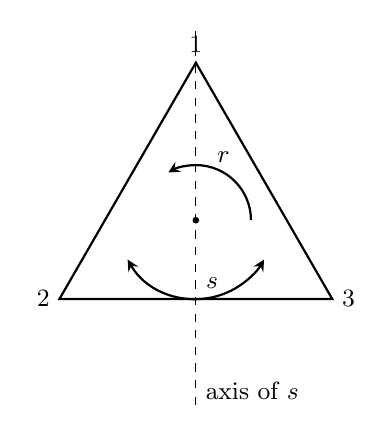
\begin{tikzpicture}[scale=2, every node/.style={font=\small}]
      % triangle vertices
      \coordinate (A) at (90:1);   % vertex 1 (top)
      \coordinate (B) at (210:1);  % vertex 2 (left)
      \coordinate (C) at (330:1);  % vertex 3 (right)
      % draw triangle
      \draw[thick] (A) -- (B) -- (C) -- cycle;
      % labels
      \node[above] at (A) {1};
      \node[left]  at (B) {2};
      \node[right] at (C) {3};

      % center
      \coordinate (O) at (0,0);
      \fill (O) circle (0.6pt);

      % dashed vertical axis (mirror axis for s)
      \draw[dashed] (0,1.2) -- (0,-1.2) node[above right] {axis of $s$};

      % small counter-clockwise rotation arrow for r
      \draw[->, >=stealth, thick] (0.35,0) arc (0:120:0.35) node[pos=0.5, above] {$r$};
      % double-headed curved arrow for s crossing the dashed axis (swap 2 <-> 3), small size
      \draw[<->, >=stealth, thick] (210:0.5) arc (210:330:0.5) node[pos=0.5, above right] {$s$};      
      \end{tikzpicture}
    \end{center}
  \end{define}



  
  \newpage
  \begin{enumerate}
    \item Find the order of every $a \in G$.
    \begin{subanswer}
      Let $G = S_3 = \{e, x, x^2, a, xa, x^2a\}$. The order of an element $g$, $o(g)$, is the smallest positive integer $m$ such that $g^m = e$.
      \begin{itemize}
        \item \textbf{Order 1:} $o(e) = 1$.
        \item \textbf{Order 2:} The elements of order 2 are the reflections.
        \begin{itemize}
          \item $o(a) = 2$, since $a^2 = e$.
          \item $o(xa) = 2$, since $(xa)^2 = (xa)(xa) = x(ax)a = x(x^2a)a = x^3a^2 = (e)(e) = e$.
          \item $o(x^2a) = 2$, since $(x^2a)^2 = (x^2a)(x^2a) = x^2(ax^2)a = x^2(xa)a = x^3a^2 = (e)(e) = e$.
        \end{itemize}
        \item \textbf{Order 3:} The elements of order 3 are the non-identity rotations.
        \begin{itemize}
          \item $o(x) = 3$, since $x^3 = e$.
          \item $o(x^2) = 3$, since $(x^2)^3 = x^6 = (x^3)^2 = e^2 = e$.
        \end{itemize}
      \end{itemize}
    \end{subanswer}

    \item Find all subgroups $H \subseteq G$. \textit{Hint: there are 6 for $S_3$}.
    \begin{subanswer}
      By Lagrange's Theorem, subgroups must have an order dividing $\abs{G}=6$. The possible orders are 1, 2, 3, and 6.
      \begin{itemize}
        \item \textbf{Order 1 (Trivial):} $H_1 = \{e\}$
        \item \textbf{Order 2 (Cyclic):} Generated by the three elements of order 2.
        \begin{itemize}
          \item $H_2 = \langle a \rangle = \{e, a\}$
          \item $H_3 = \langle xa \rangle = \{e, xa\}$
          \item $H_4 = \langle x^2a \rangle = \{e, x^2a\}$
        \end{itemize}
        \item \textbf{Order 3 (Cyclic):} Generated by the two elements of order 3.
        \begin{itemize}
          \item $H_5 = \langle x \rangle = \langle x^2 \rangle = \{e, x, x^2\}$
        \end{itemize}
        \item \textbf{Order 6 (The group itself):} $H_6 = G = \{e, x, x^2, a, xa, x^2a\}$
      \end{itemize}
    \end{subanswer}

    \item Identify $Z(G)$. Identify $\langle a \rangle$ and $C(a)$ for each $a \in G$.
    \begin{subanswer}
      \begin{itemize}
        \item \textbf{Center $Z(G)$:} The set of elements that commute with all 
        elements in $G$. Since $xa = ax^2 \neq ax$, $x$ does not commute with 
        $a$. Since the group is non-abelian, the center is a proper subgroup. 
        A quick check shows that only the identity commutes with all 6 elements.
          \[ Z(G) = \{e\} \]
        \item \textbf{Cyclic Subgroups $\langle a \rangle$:}
          \begin{itemize}
            \item $\langle e \rangle = \{e\}$
            \item $\langle x \rangle = \langle x^2 \rangle = \{e, x, x^2\}$
            \item $\langle a \rangle = \{e, a\}$
            \item $\langle xa \rangle = \{e, xa\}$
            \item $\langle x^2a \rangle = \{e, x^2a\}$
          \end{itemize}
        \item \textbf{Centralizers $C(a) = \{g \in G \mid ga = ag\}$:}
          \begin{itemize}
            \item $C(e) = G$
            \item $C(x) = \{g \mid gx = xg\}$. The elements that commute with $x$ are $e, x, x^2$.
              \[ C(x) = \{e, x, x^2\} \]
            \item $C(x^2) = \{g \mid gx^2 = x^2g\}$. Since $g$ commutes with $x^2$ iff it commutes with $x$,
              \[ C(x^2) = \{e, x, x^2\} \]
            \item $C(a) = \{g \mid ga = ag\}$. Only $e$ and $a$ commute with $a$.
              \[ C(a) = \{e, a\} \]
            \item $C(xa) = \{g \mid g(xa) = (xa)g\}$. Only $e$ and $xa$ commute with $xa$.
              \[ C(xa) = \{e, xa\} \]
            \item $C(x^2a) = \{g \mid g(x^2a) = (x^2a)g\}$. Only $e$ and $x^2a$ commute with $x^2a$.
              \[ C(x^2a) = \{e, x^2a\} \]
          \end{itemize}
      \end{itemize}
    \end{subanswer}

    \item For each subgroup $H$, find the equivalence classes under the relation $R_H$ in problem 6.
    \begin{subanswer}
      The relation is $(a, b) \in R_H$ if $ab^{-1} \in H$. The equivalence classes $[a] = \{b \mid ab^{-1} \in H\}$ are the \textbf{right cosets $Ha = \{ha \mid h \in H\}$}.
      \begin{itemize}
        \item \textbf{$H_1 = \{e\}$:} The cosets are the elements themselves.
          \begin{itemize}
            \item $[e] = \{e\}$, $[x] = \{x\}$, $[x^2] = \{x^2\}$, $[a] = \{a\}$, $[xa] = \{xa\}$, $[x^2a] = \{x^2a\}$
          \end{itemize}
        \item \textbf{$H_2 = \{e, a\}$:}
          \begin{itemize}
            \item $H_2e = \{e \cdot e, a \cdot e\} = \{e, a\}$
            \item $H_2x = \{e \cdot x, a \cdot x\} = \{x, ax\} = \{x, x^2a\}$
            \item $H_2x^2 = \{e \cdot x^2, a \cdot x^2\} = \{x^2, ax^2\} = \{x^2, xa\}$
          \end{itemize}
        \item \textbf{$H_3 = \{e, xa\}$:}
          \begin{itemize}
            \item $H_3e = \{e, xa\}$
            \item $H_3x = \{x, (xa)x\} = \{x, a\}$
            \item $H_3x^2 = \{x^2, (xa)x^2\} = \{x^2, x^2a\}$
          \end{itemize}
        \item \textbf{$H_4 = \{e, x^2a\}$:}
          \begin{itemize}
            \item $H_4e = \{e, x^2a\}$
            \item $H_4x = \{x, (x^2a)x\} = \{x, xa\}$
            \item $H_4x^2 = \{x^2, (x^2a)x^2\} = \{x^2, a\}$
          \end{itemize}
        \item \textbf{$H_5 = \{e, x, x^2\}$:} (This is a normal subgroup)
          \begin{itemize}
            \item $H_5e = \{e \cdot e, x \cdot e, x^2 \cdot e\} = \{e, x, x^2\}$
            \item $H_5a = \{e \cdot a, x \cdot a, x^2 \cdot a\} = \{a, xa, x^2a\}$
          \end{itemize}
        \item \textbf{$H_6 = G$:}
          \begin{itemize}
            \item $H_6e = G = \{e, x, x^2, a, xa, x^2a\}$
          \end{itemize}
      \end{itemize}
    \end{subanswer}

    \item For each $a \in G$, find its equivalence class under the relation $R$ from problem 7.
    \begin{subanswer}
      The relation is $(a, b) \in R$ if $b = g^{-1} a g$ for some $g \in G$. These are the \textbf{conjugacy classes}.
      \begin{itemize}
        \item \textbf{$[e]$:} The class of the identity is always just the identity.
          \[ [e] = \{g^{-1}eg \mid g \in G\} = \{e\} \]
        \item \textbf{$[x]$:} The class of rotations.
          \begin{itemize}
            \item $e^{-1}xe = x$
            \item $x^{-1}xx = x$
            \item $(x^2)^{-1}xx^2 = x(x)x^2 = x^4 = x$
            \item $a^{-1}xa = axa = a(ax^2) = x^2$
            \item $(xa)^{-1}x(xa) = (xa)x(xa) = (xa)(x^2a) = x(a x^2 a) = x(a(xa)) = x(x) = x^2$
            \item $(x^2a)^{-1}x(x^2a) = (x^2a)x(x^2a) = (xa)(x^2a) = x(ax^2a) = x(a(xa)) = x(x) = x^2$
          \end{itemize}
          \[ [x] = \{x, x^2\} \]
        \item \textbf{$[x^2]$:} Since $x^2 \in [x]$, $[x^2] = [x] = \{x, x^2\}$.
        \item \textbf{$[a]$:} The class of reflections.
          \begin{itemize}
            \item $e^{-1}ae = a$
            \item $x^{-1}ax = x^2(ax) = x^2(x^2a) = x^4a = xa$
            \item $(x^2)^{-1}ax^2 = x(ax^2) = x(xa) = x^2a$
          \end{itemize}
          (All other conjugates will also land in this set).
          \[ [a] = \{a, xa, x^2a\} \]
        \item \textbf{$[xa]$:} Since $xa \in [a]$, $[xa] = [a] = \{a, xa, x^2a\}$.
        \item \textbf{$[x^2a]$:} Since $x^2a \in [a]$, $[x^2a] = [a] = \{a, xa, x^2a\}$.
      \end{itemize}
      The distinct conjugacy classes are: $\{e\}$, $\{x, x^2\}$, and $\{a, xa, x^2a\}$.
    \end{subanswer}
  \end{enumerate}
  

  \newpage
  \item Repeat problem 8 where $G=D_8$, the dihedral group of order 8. 
  \textit{Hint: there are 10 subgroups}.
  \begin{enumerate}
    \item Find the order of every $a \in G$.
    \begin{subanswer}
      The elements of $D_8$ are: $e$, $r$, $r^2$, $r^3$, $s$, $sr$, $sr^2$, $sr^3$.
      \begin{itemize}
        \item $o(e) = 1$
        \item $o(r) = 4$
        \item $o(r^2) = 2$
        \item $o(r^3) = 4$
        \item $o(s) = 2$
        \item $o(sr) = 2$
        \item $o(sr^2) = 2$
        \item $o(sr^3) = 2$
      \end{itemize}
    \end{subanswer}
    \item Find all subgroups $H \subseteq G$. \textit{Hint: there are 6 for $S_3$}.
    \begin{subanswer}
      The subgroups of $D_8$ are:
      \begin{itemize}
        \item $H_1 = \{e\}$
        \item $H_2 = \{e, r^2\}$
        \item $H_3 = \{e, r, r^2, r^3\}$
        \item $H_4 = \{e, s\}$
        \item $H_5 = \{e, sr^2\}$
        \item $H_6 = D_8$
      \end{itemize}
    \end{subanswer}
    \item Identify $Z(G)$. Identify $(a)$ and $C(a)$ for each $a \in G$.
    \begin{subanswer}
      The center $Z(G)$ consists of all elements that commute with every element of $G$. In $D_8$, we have:
      \begin{itemize}
        \item $Z(D_8) = \{e, r^2\}$
      \end{itemize}
      The centralizer $C(a)$ for each $a \in G$ is:
      \begin{itemize}
        \item $C(e) = D_8$
        \item $C(r) = \{e, r, r^2, r^3\}$
        \item $C(r^2) = D_8$
        \item $C(r^3) = \{e, r, r^2, r^3\}$
        \item $C(s) = \{e, s\}$
        \item $C(sr) = \{e, sr\}$
        \item $C(sr^2) = \{e, sr^2\}$
        \item $C(sr^3) = \{e, sr^3\}$
      \end{itemize}
    \end{subanswer}
    \item For each subgroup $H$, find the equivalence classes under the relation $R_H$ in problem 6.
    \begin{subanswer}
      The equivalence classes under the relation $R_H$ are:
      \begin{itemize}
        \item For $H_1 = \{e\}$: Each element forms its own class.
        \item For $H_2 = \{e, r^2\}$: Classes are $\{e, r^2\}$, $\{r, r^3\}$, $\{s, sr^2\}$, $\{sr, sr^3\}$.
        \item For $H_3 = \{e, r, r^2, r^3\}$: Classes are $\{e, r, r^2, r^3\}$ and $\{s, sr, sr^2, sr^3\}$.
        \item For $H_4 = \{e, s\}$: Classes are $\{e, s\}$, $\{r, sr\}$, $\{r^2, sr^2\}$, $\{r^3, sr^3\}$.
        \item For $H_5 = \{e, sr^2\}$: Classes are $\{e, sr^2\}$, $\{r, sr^3\}$, $\{r^2, s\}$, $\{r^3, sr\}$.
        \item For $H_6 = D_8$: The entire group is one class.
      \end{itemize}
    \end{subanswer}
    \item For each $a \in G$, find its equivalence class under the relation $R$ from problem 7.
    \begin{subanswer}
      The conjugacy classes in $D_8$ are:
      \begin{itemize}
        \item $[e] = \{e\}$
        \item $[r] = \{r, r^3\}$
        \item $[r^2] = \{r^2\}$
        \item $[s] = \{s, sr^2\}$
        \item $[sr] = \{sr, sr^3\}$
      \end{itemize}
      The conjugacy classes partition the group $D_8$ into disjoint subsets.
    \end{subanswer}
  \end{enumerate}

  \newpage
  \item Repeat problem 8 where $G=\left(\setZ_n,+\right)$ for 
  $n=3,4,5,6$ and for $V_4$ from problem 1.
  \begin{enumerate}
    \item Find the order of every $a \in G$.
    \begin{subanswer}
      The elements of $\setZ_n$ are $\{[0], [1], [2], \ldots, [n-1]\}$. 
      The order of each element is:
      \begin{itemize}
        \item For $n=3$: $o([0])=1$, $o([1])=3$, $o([2])=3$.
        \item For $n=4$: $o([0])=1$, $o([1])=4$, $o([2])=2$, $o([3])=4$.
        \item For $n=5$: $o([0])=1$, $o([1])=5$, $o([2])=5$, $o([3])=5$, $o([4])=5$.
        \item For $n=6$: $o([0])=1$, $o([1])=6$, $o([2])=3$, $o([3])=2$, $o([4])=3$, $o([5])=6$.
      \end{itemize}
      The orders of the elements in $\setZ_n$ are determined by the divisors of $n$.
    \end{subanswer}
    \item Find all subgroups $H \subseteq G$. \textit{Hint: there are 6 for $S_3$}.
    \begin{subanswer}
      The subgroups of $\setZ_n$ are:
      \begin{itemize}
        \item For $n=3$: $\{[0]\}$, $\{[0], [1], [2]\}$.
        \item For $n=4$: $\{[0]\}$, $\{[0], [2]\}$, $\{[0], [1], [2], [3]\}$.
        \item For $n=5$: $\{[0]\}$, $\{[0], [1], [2], [3], [4]\}$.
        \item For $n=6$: $\{[0]\}$, $\{[0], [2], [4]\}$, $\{[0], [1], [2], [3], [4], [5]\}$.
      \end{itemize}
      The subgroup structure is determined by the divisors of $n$.
    \end{subanswer}
    \item Identify $Z(G)$. Identify $(a)$ and $C(a)$ for each $a \in G$.
    \begin{subanswer}
      Since $\setZ_n$ is abelian, $Z(G) = G$ for all $n$.
      The cyclic subgroup generated by each element $[a]$ is 
      $\langle [a] \rangle = \{[ka] \mid k \in \setZ\}$.
      The centralizer $C([a]) = G$ for all $[a]$ since the group is abelian.
    \end{subanswer}
    \item For each subgroup $H$, find the equivalence classes under the relation $R_H$ in problem 6.
    \begin{subanswer}
      The equivalence classes under the relation $R_H$ are the cosets of $H$ in $G$.
      Since $\setZ_n$ is abelian, the left and right cosets coincide.
      For each subgroup $H$, the cosets partition $G$ into disjoint subsets.
      The equivalence classes are:
      \begin{itemize}
        \item For $n=3$: $\{[0]\}$, $\{[1], [2]\}$.
        \item For $n=4$: $\{[0]\}$, $\{[2]\}$, $\{[1], [3]\}$.
        \item For $n=5$: $\{[0]\}$, $\{[1], [2], [3], [4]\}$.
        \item For $n=6$: $\{[0]\}$, $\{[2], [4]\}$, $\{[1], [3], [5]\}$.
      \end{itemize}
    \end{subanswer}
    \item For each $a \in G$, find its equivalence class under the relation $R$ from problem 7.
    \begin{subanswer}
      Since $\setZ_n$ is abelian, each element forms its own conjugacy class.
      Thus, for each $[a] \in \setZ_n$, the equivalence class is:
      \[
        [ [a] ] = \{ [a] \}
      \]
      for all $n=3,4,5,6$.
    \end{subanswer}
  \end{enumerate}
\end{enumerate}


























\newpage\handout[true]
{\textsc{Math 2106-B: Foundations of Mathematical Proof}}{Fall 2025}
{Homework 7: Groups and Subgroups}
{\textit{Prof.} \href{https://ceheitsch.github.io/webpage/}{Dr. Christine Heitsch}}{Due Date: October 30, 2025}
{Math 2106-B: HW7}
{\large
  \noindent
  \textbf{Name:} \HandoutAuthor \smallskip \\

  \noindent
  \textbf{GTID:} 903743506 \smallskip \\

  \noindent
  %%% List anyone with whom you discussed the problems
  \textbf{Collaborators:} None. This material reflects independent preparation. \smallskip \\

  \noindent
  %%% List all resources used OTHER than the textbook, lecture notes, 
  %%% webwork problems, ICA questions, and previous homework assignments.
  \textbf{Outside resources:} This work was informed by MATH 2106 course materials 
  (ICAs: in-class activities and WebWork contents) from \HandoutInstitution\ (the course textbook is 
  Chartrand \parencite{chartrand_mathematical_2018}).   
  Outside references specifically include
  textbooks written by 
  Grimaldi \parencite{grimaldi_discrete_2004} (used in MATH 3012) and 
  Rosen \parencite{rosen_discrete_2019} (used in CS 2050). \smallskip \\

  \noindent
  \textbf{Notice}: The answers contain cross-references throughout this document as clickable hyperlinks in most PDF viewers. However, the Gradescope PDF view might not support clickable hyperlinks.
}
\printbibliography[
  heading=bibintoc,   
  title={References}     % change “References” text if needed
]
% `heading=bibnumbered` if you prefer it numbered chapter (in \tableofcontents)
% `heading=bibintoc`    if you prefer it unnumbered but still in the ToC
\newpage
% \printbibliography[
  heading=bibintoc,   
  title={References}     % change “References” text if needed
]
% `heading=bibnumbered` if you prefer it numbered chapter (in \tableofcontents)
% `heading=bibintoc`    if you prefer it unnumbered but still in the ToC\newpage
% The following table presents the standard logical equivalences from these sources together with 
the author's own (or the student, myself, Jaehoon Song) clarifications and labels where applicable.


\begin{table}[h!]
  \centering
  \renewcommand{\arraystretch}{1.2}
  \setlength{\tabcolsep}{8pt}
  \begin{tabular}{|p{5.0cm}|p{5.0cm}|p{5.2cm}|}
    \hline
    \rowcolor[HTML]{E0E0E0}
    \multicolumn{2}{|l|}{\textbf{Logical Equivalences}} & \textbf{Name} \\
    \hline
    $\,p \AND q \equiv q \AND p$ & $\,p \OR q \equiv q \OR p$ & Commutative Law \\
    \hline
    $\, (p \AND q) \AND r \equiv p \AND (q \AND r)$ & $\, (p \OR q) \OR r \equiv p \OR (q \OR r)$ & Associative Law \\
    \hline
    $\,p \AND (q \OR r) \equiv (p \AND q) \OR (p \AND r)$ & $\,p \OR (q \AND r) \equiv (p \OR q) \AND (p \OR r)$ & Distributive Law \\
    \hline
    $\,\overline{p \AND q} \equiv \sNOT{p} \OR \sNOT{q}$ & $\,\overline{p \OR q} \equiv \sNOT{p} \AND \sNOT{q}$ & DeMorgan's Law \\
    \hline
    \multicolumn{2}{|l|}{$\,\overline{\overline{p}} \equiv p$} & Double Negation law \\
    \hline
    $\,p \AND \boldsymbol{T} \equiv p$ & $\,p \OR \boldsymbol{F} \equiv p$ & Identity Law \\
    \hline
    $\,p \OR \boldsymbol{T} \equiv \boldsymbol{T}$ & $\,p \AND \boldsymbol{F} \equiv \boldsymbol{F}$ & Domination Law \\
    \hline
    $\,p \AND p \equiv p$ & $\,p \OR p \equiv p$ & Idempotent Law \\
    \hline
    \multicolumn{2}{|l|}{$\,p \THEN q \equiv \sNOT{p} \OR q$} & Implication Equivalence \\
    \hline
    \multicolumn{2}{|l|}{$\,\overline{p \THEN q} \equiv p \AND \sNOT{q}$} & Negation of Implication \\
    \hline
    \multicolumn{2}{|l|}{$\,p \THEN q \equiv \sNOT{q} \THEN \sNOT{p}$} & Contrapositive Equivalence \\
    \hline
    \multicolumn{2}{|l|}{$\,p \OR \sNOT{p} \equiv \boldsymbol{T}$} & Law of Tautology \\
    \hline
    \multicolumn{2}{|l|}{$\,p \AND \sNOT{p} \equiv \boldsymbol{F}$} & Law of Contradiction \\
    \hline
  \end{tabular}
\end{table}\newpage
% 
The following definitions are presented from standard mathematical sources (\textbf{Sets}).
Clarifications and labels have been added where applicable.

\begin{define}{Basic Set Concepts}\phantomsection\label{def:basic-set-concepts} % \hyperref[def:basic-set-concepts]{YOUR_CONTEXT}
  \begin{enumerate}
    \item \textbf{Universal Set:} A universal set $\setUNIV$ is a
    set that contains all objects under consideration in a particular context or problem.
    \item \textbf{Empty Set:} The empty set, denoted $\setNULL$,
    is the unique set that contains no elements.
    \item \textbf{Subset:} Let $A$ and $B$ be sets. $A$ is a
    subset of $B$ ($A \subseteq B$) if (and only if)
    for all $x \in A$, $x \in B$.
    \item \textbf{Set Equality:} Let $A$ and $B$ be sets. The sets $A$ and $B$ are
    equal ($A = B$) if $A \subseteq B$ and $B \subseteq A$.
    \item \textbf{Power Set:} Let $A$ be a set. The power set of $A$, denoted $\sPOWER{A}$ or $2^A$,
    is the set of all subsets of $A$. That is, $\mathcal{P}(A) = \{S\in\setUNIV : S \subseteq A\}$.
  \end{enumerate}
\end{define}
The following definitions extend the understanding of set operations
and properties.


\begin{define}{Set Operations}\phantomsection\label{def:set-operations} % \hyperref[def:set-operations]{YOUR_CONTEXT}
  \begin{enumerate}
    \item \textbf{Complementary Set:} Let $A$ be a subset of the universal set $\setUNIV$.
    The complement of $A$, denoted $A^c$ or $\overline{A}$, is the set of all elements
    in $\setUNIV$ that are not in $A$. That is, $A^c = \{x \in \setUNIV : x \notin A\}$.
    \item \textbf{Union:} Let $A$ and $B$ be sets. The union of $A$ and $B$,
    denoted $A \cup B$, is the set of all elements that are in $A$, or in $B$, or in both.
    That is, $A \cup B = \{x : x \in A \lor x \in B\}$.
    \item \textbf{Intersection:} Let $A$ and $B$ be sets. The intersection of $A$ and $B$,
    denoted $A \cap B$, is the set of all elements that are in both $A$ and $B$.
    That is, $A \cap B = \{x : x \in A \land x \in B\}$.
    \item \textbf{Set Difference:} Let $A$, $B$ be subsets of a universal set $\setUNIV$.
    The set difference $A \sMINUS B$ is defined to be the set
    $\{ x \in \setUNIV \LDIV x \in A \text{ and } x \notin B\}$. \vspace*{10px}\\
    \textit{It is sometimes called the relative complement of $B$ in $A$,
    and denoted in the textbook as $A - B$.}
    \item \textbf{Cartesian Product:} Let $A$ and $B$ be sets. The Cartesian product of
    $A$ and $B$, denoted $A \sTIMES B$, is the set consisting of all ordered pairs:
    \[
    A \sTIMES B = \{(a, b) \LDIV a \in A, b \in B\}.
    \]
  \end{enumerate}
\end{define}


\newpage

The following claims are given in the reference as well. Let $A,B\in U$, a universal set.


\begin{claim}{Subset of Union: $A \subseteq \sOR{A}{B}$}\phantomsection\label{claim:subset-union} % \hyperref[claim:subset-union]{YOUR_CONTEXT}
  \begin{subprove}[bluecolor]
      Let $x\in U$, assume $x\in A$. Then the statement \inlinequote{$x\in A$ or $x\in B$} is true.
      Hence, by the definition, $\sOR{A}{B}=\{x\in U\LDIV x\in A$ or $x\in B\}$, $x\in \sOR{A}{B}$.
      Thus, $A \subseteq \sOR{A}{B}$.
  \end{subprove}
\end{claim}

\begin{claim}{Empty Subset: $\setNULL \subseteq A$}\phantomsection\label{claim:empty-subset} % \hyperref[claim:empty-subset]{YOUR_CONTEXT}
  \begin{subprove}[bluecolor]
      Let $x\in U$, assume $x\in \setNULL$. But there are no elements in $\setNULL$, so
      $x\in \setNULL$ is false. Since the premise is false, the implication if $x\in \setNULL$,
      then $x\in A$ is true. Thus, $\setNULL \subseteq A$ by definition of \hyperref[def:basic-set-concepts]{subsets}.
  \end{subprove}
\end{claim}

\begin{claim}{Subset as Equality: $\sOR{A}{B}=A$ if and only if $B\subseteq A$}\phantomsection\label{claim:subset-equality} % \hyperref[claim:subset-equality]{YOUR_CONTEXT}
  \begin{subprove}[bluecolor]
      Let $x\in U$, first, we assume $B\subseteq A$, we have already shown
      $A \subseteq \sOR{A}{B}$ by the claim, \hyperref[claim:subset-union]{Subset of Union}. 
      To show $\sOR{A}{B} \subseteq A$, assume $x\in \sOR{A}{B}$.
      By definition, $x\in A$ or $x\in B$. Considering $x\in B$ and assumption
      $B \subseteq A$, $x\in B$ implies $x\in A$. Thus, $\sOR{A}{B} \subseteq A$.
      Hence, if $B\subseteq A$, then $\sOR{A}{B} = A$. \vspace*{10px}\\
      Now, we assume $\sOR{A}{B}=A$. To show $B\subseteq A$, we now assume $x\in B$. Since $x\in B$, by definition
      of union, $x\in \sOR{A}{B} = A$. Therefore, $B\subseteq A$.
  \end{subprove}
\end{claim}


%%%%%%%%%%%%%%%%%%% 9/8/25

Let $\setUNIV$ be a set. 
\begin{claim}{ICA6}\phantomsection\label{claim:ica6} % \hyperref[claim:ica6]{YOUR_CONTEXT}
  For all $A,B\in\setUNIV$, $$A\sTIMES B =\setNULL\THEN \group{A=\setNULL\OR B=\setNULL}$$
  \begin{subprove}[bluecolor]
    Let $A,B\in\setUNIV$. We prove $A\sTIMES B=\setNULL$. Assume it is not the case that 
    $A=\setNULL$ or $B=\setNULL$. Thus, we have $A=\setNULL$ and $B=\setNULL$. 
    Since $A\ne\setNULL$ by assumption, there exists an element $a\in A$. Likewise, there 
    is some $b\in B$ since $B\ne\setNULL$. Thus, $\group{a,b}\in\sBUILD{(x,y)}{x\in A,y\in B}$ 
    by definition. But then, $A\sTIMES B\ne\setNULL$ by definition. Hence, the claim holds. 
  \end{subprove}
\end{claim}


\begin{define}{Relatively Prime Integers (Coprime)}\phantomsection\label{def:relatively-prime} % \hyperref[def:relatively-prime]{YOUR_CONTEXT}
  Let $x,y \in \mathbb{Z}$. The integers $x$ and $y$ are said to be
  \textbf{relatively prime} if and only if
  $\gcd(x,y) = 1$.
\end{define}
\newpage
% The following definitions and axioms are presented from standard mathematical sources (\textbf{Number Theory}) together with the author's own (or the student, myself, Jaehoon Song) clarifications and labels where applicable.

\begin{define}{Integers}[def:integers][red]
  $\setZ$: the set of all integers
\end{define}

\begin{define}{Rational Numbers}[def:rational-numbers][red]
  $\setQ$: the set of all rational numbers
\end{define}

\begin{define}{Real Numbers}[def:real-numbers][red]
  $\setR$: the set of all real numbers
\end{define}

\begin{define}{Natural Numbers}[def:natural-numbers][red]
  $\setN$ or $\setZ_{>0}$: the set of all natural numbers which are the set of positive integers (not including $0$)
\end{define}

\begin{define}{Positive Real Numbers}[def:positive-real-numbers][red]
  $\setR_{>0}$: the set of all positive real numbers
\end{define}

\begin{define}{Non-negative Real Numbers}[def:non-negative-real-numbers][red]
  $\setR_{\geq 0}$: the set of all non-negative real numbers
\end{define}


\newpage

The following definitions and claims extend the understanding of integers.

Here are the ICA2 Definitions and Axioms as follows.

\begin{define}{Even Integer}[def:even-integer][red]
  An integer $n$ is \underbar{even} if there exists 
  (existential quantification logic $\exists$) an integer $k$ such that
  \[
  n = 2k.
  \]
\end{define}

\begin{define}{Odd Integer}[def:odd-integer][red]
  An integer $n$ is \underbar{odd} if 
  there exists some integer $k$ such that
  \[
  n = 2k + 1.
  \]
\end{define}

\begin{define}{Closure under Addition}[def:closure-addition][red]
  The sum of two integers is again an 
  integer. (Closure under addition)
\end{define}

\begin{define}{Closure under Multiplication}[def:closure-multiplication][red]
  The product of two integers is again 
  an integer. (Closure under multiplication)
\end{define}

\begin{define}{Odd if and only if Not Even}[def:odd-iff-not-even][red]
  An integer is odd if and only if it 
  is not even.
\end{define}

Here are the ICA3 Definitions and Axioms as follows.

\begin{define}{Universal Closure under Addition}[def:universal-closure-addition][red]
  The sum of two integers (Universal quantification for all, for every, for each) is again an integer. (Closure under addition)
\end{define}

\begin{define}{Universal Closure under Multiplication}[def:universal-closure-multiplication][red]
  The product of two integers (Universal quantification for all, for every, for each) is again an integer. (Closure under multiplication)
\end{define}

\begin{define}{Even Integer Square}[def:even-integer-square][red]
  An integer $n$ is even if and only if $n^2$ is even.
\end{define}

\newpage

The following claims are given in the reference as well.

\begin{define}{Sum of Even Integers}[claim:sum-even-integers][red]
  The sum of two even integers is again an even integer.
  \begin{subprove}[red]
    Let $x$ be an integer and $y$ be an integer ($\forall x,y \in \setZ$). 
    Suppose $x$ is even and $y$ is even. Then, by \nameref{def:even-integer}, there exists an integer 
    $k$ and an integer $j$ such that $x=2k$ and $y=2j$. Then, 
    $x+y=\left(2k\right)+\left(2j\right)=2\left(k+j\right)$. By \nameref{def:closure-addition}, since $k$ and 
    $j$ are integers, then so is $\left(k+j\right)$. Hence, by definition, $x+y$ is an 
    even integer.
  \end{subprove}
\end{define}

The following definitions extend the understanding of integers including divisibility.

\begin{define}{Divisibility}[def:divisibility][red]
  An integer $n$ divides an integer $m$, denoted $n \LDIV m$, if there 
  exists an integer $k$ such that $m=n k$. Otherwise, $n \nmid m$.
\end{define}

The following definitions extend the classification of real numbers into rational and irrational numbers.

\begin{define}{Rational Number}[def:rational-number][red]
  A real number $x$ is \underbar{rational} if there exist integers $a$ and $b$ with $b \neq 0$ such that $bx = a$.
  Otherwise, $x$ is \underbar{irrational}.

  \textbf{Note}: Compare the rational number definition with the even/odd axiom \inlinequote{odd iff not even} from \nameref{def:odd-iff-not-even}.
\end{define}

The following claims are given in the reference as well.

\begin{define}{Irrationality of $\sqrt{2}$}[claim:sqrt2-irrational][red]
  $\sqrt{2}$ is irrational.
  \begin{subprove}[red]
    Suppose $\sqrt{2}$ is rational. Then, by \nameref{def:rational-number}, there exists $a,b\in \setZ$ 
    with $b\ne 0$ such that $b\cdot\sqrt{2}=a$. We may further assume that any factors 
    common to $a$ and $b$ have already been removed.\\

    Then, squaring both sides, this yields $2\cdot b^2 = a^2$.
    Since products of integers are again integers by \nameref{def:closure-multiplication}, we have that $a^2,b^2\in \setZ$.
    Thus, by definition, $a^2$ is even. Therefore, by \nameref{def:even-integer-square}, $a$ is even. 
    Thus, there exists $c\in\setZ$ such that $a=2c$. Then
    $$
    2b^2=a^2={2c}^2=4c^2
    $$
    Then, $b^2=2c^2$. Then, as before, $b^2$ is even, so $b$ is even.
    However, $a$ and $b$ both being even contradicts the fact that any factors 
    common to $a$ and $b$ have already been removed.
  \end{subprove}
\end{define}






%%%%%%%%%%%%%%%%%%% New style (refactor model)
\begin{define}{Relatively Prime Integers (Coprime)}[def:relatively-prime][red]
  Let $x,y \in \mathbb{Z}$. The integers $x$ and $y$ are said to be
  \textbf{relatively prime} if and only if
  $\gcd(x,y) = 1$.
\end{define}\newpage
%%%%%%%%%%%%%%%%%%%%%%%%%%%%%%%%%%%%%%%%%%%%%%%%%%%%%%%%%%%%%%%%%%%%%%%
% References Section
%%%%%%%%%%%%%%%%%%%%%%%%%%%%%%%%%%%%%%%%%%%%%%%%%%%%%%%%%%%%%%%%%%%%%%%
\textbf{Remark}: The following definitions (or results) are already proved in class or on previous ICA, 
Wbwk, Hmwk assignments, and contents of the textbook.





%%%%%%%%%%%%%%%%%%%%%%%%%%%%%%%%%%%%%%%%%%%%%%%%%%%%%%%%%%%%%%%%%%%%%%%
% Problems Section
%%%%%%%%%%%%%%%%%%%%%%%%%%%%%%%%%%%%%%%%%%%%%%%%%%%%%%%%%%%%%%%%%%%%%%%
\newpage
Let $G$ be a group with identity $e$.
\begin{enumerate}
  \item Prove or disprove from the definitions:
  \begin{enumerate}
    \item A cyclic group is abelian.
    \begin{define}{Cyclic Group}[def:cyclic-group][red]
      A group $(G, *)$ is called a \textbf{cyclic group} if there exists an element $g \in G$ such that $G = (g) = \{g^i \mid i \in \setZ\}$, 
      where $(g)$ is the cyclic subgroup generated by $g$ as defined in \nameref{def:cyclic-subgroup}. 
      The element $g$ is called a \textbf{generator} of $G$.
    \end{define}
    \begin{subprove}
      Let $(G, *)$ be a cyclic group and let $g \in G$ be a generator of $G$ such that $G = (g) = \{g^i \mid i \in \setZ\}$.
      Let $a, b \in G$ be arbitrary elements.
      Since $G$ is cyclic, there exist integers $m, n \in \setZ$ such that $a = g^m$ and $b = g^n$.
      By the properties of exponentiation,
      \[
        a * b = g^m * g^n = g^{m+n} = g^{n+m} = g^n * g^m = b * a.
      \]
      Since $a$ and $b$ were arbitrary elements of $G$, it follows that for all $a, b \in G$, $a * b = b * a$.
      Therefore, by definition of \nameref{def:abelian-group}, $G$ is an abelian group.
    \end{subprove}
    \item An abelian group is cyclic.
    \begin{subprove}
      This statement is disproved by the following counterexample.
      
      Let $V_4 = \setZ_2 \times \setZ_2$ be the Klein 4-group under coordinate-wise addition, 
      which was shown to be an abelian group in Homework 6.
      The elements of $V_4$ are $\{([0],[0]), ([0],[1]), ([1],[0]), ([1],[1])\}$.
      
      For $V_4$ to be cyclic, there must exist an element $g \in V_4$ such that $(g) = V_4$.
      However, it is observed that:
      \begin{itemize}
        \item The element $([0],[0])$ is the identity and generates only itself.
        \item The element $([0],[1])$ satisfies $([0],[1])^2 = ([0],[0])$, so $( ([0],[1]) ) = \{([0],[0]), ([0],[1])\}$.
        \item The element $([1],[0])$ satisfies $([1],[0])^2 = ([0],[0])$, so $( ([1],[0]) ) = \{([0],[0]), ([1],[0])\}$.
        \item The element $([1],[1])$ satisfies $([1],[1])^2 = ([0],[0])$, so $( ([1],[1]) ) = \{([0],[0]), ([1],[1])\}$.
      \end{itemize}
      Since no element generates all four elements of $V_4$, it is concluded that $V_4$ is not cyclic.
      
      Therefore, since $V_4$ is an abelian group that is not cyclic, the statement that an abelian group is cyclic is disproved.
    \end{subprove}
  \end{enumerate}




  \newpage
  \item If $G$ is cyclic, prove that every subgroup of $G$ is cyclic.
  \begin{subprove}
    Let $(G, *)$ be a cyclic group with generator $g \in G$ such that $G = (g) = \{g^i \mid i \in \setZ\}$.
    Let $H$ be a subgroup of $G$ for the sake of direct proof.
    
    Two cases are considered.
    
    \textbf{Case 1:} If $H = \{e\}$, where $e$ is the identity element of $G$, then $H$ is cyclic since it is generated by $e$.
    
    \textbf{Case 2:} If $H \neq \{e\}$, then $H$ contains at least one non-identity element.
    Since $H \subseteq G = (g)$ and $H \neq \{e\}$, there exists an integer $k \neq 0$ such that $g^k \in H$.
    
    By the well-ordering principle, let $d$ be the smallest positive integer such that $g^d \in H$.
    It is claimed that $H = (g^d)$.
    
    To show that $H \subseteq (g^d)$, let $h \in H$ be arbitrary.
    Since $h \in H \subseteq G = (g)$, there exists an integer $n \in \setZ$ such that $h = g^n$.
    By the division algorithm, there exist integers $q$ and $r$ with $0 \leq r < d$ such that $n = qd + r$.
    It follows that
    \[
      h = g^n = g^{qd + r} = (g^d)^q * g^r.
    \]
    Since $g^d \in H$ and $H$ is a subgroup, $(g^d)^q \in H$ by closure under the group operation.
    Moreover, since $h \in H$ and $(g^d)^q \in H$, it follows that $g^r = h * ((g^d)^q)^{-1} \in H$ by closure and existence of inverses in $H$.
    
    However, since $d$ is the smallest positive integer such that $g^d \in H$ and $0 \leq r < d$, 
    the only possibility is that $r = 0$.
    Therefore, $h = (g^d)^q \in (g^d)$.
    Since $h$ was arbitrary, it is concluded that $H \subseteq (g^d)$.
    
    To show that $(g^d) \subseteq H$, since $g^d \in H$ and $H$ is a subgroup, 
    it follows by closure under the group operation that $(g^d) = \{(g^d)^i \mid i \in \setZ\} \subseteq H$.
    
    Therefore, $H = (g^d)$, and hence $H$ is cyclic by definition of \nameref{def:cyclic-group}.
    
    In both cases, it is shown that $H$ is cyclic.
    Since $H$ was an arbitrary subgroup of $G$, it follows that every subgroup of $G$ is cyclic.
  \end{subprove}





  \newpage
  
  \item A subgroup is \textit{proper} if it is neither the identity 
  nor the entire group. Prove that if $G$ has no proper subgroups, 
  then $G$ is cyclic. \textit{Do not assume that $G$ is finite}.
  \begin{define}{Proper Subgroup}[def:proper-subgroup][red]
    A subgroup $H$ of $G$ is called a \textbf{proper subgroup} if $H \neq \{e\}$ and $H \neq G$, 
    where $e$ is the identity element of $G$.
  \end{define}
  \begin{subprove}
    Let $(G, *)$ be a group with identity $e$ and suppose that $G$ has no proper subgroups for the sake of direct proof.
    
    Two cases are considered.
    
    \textbf{Case 1:} If $G = \{e\}$, then $G$ is cyclic since it is generated by $e$.
    
    \textbf{Case 2:} If $G \neq \{e\}$, then $G$ contains at least one non-identity element.
    Let $g \in G$ be an arbitrary non-identity element, i.e., $g \neq e$.
    
    Consider the cyclic subgroup $(g) = \{g^i \mid i \in \setZ\}$ generated by $g$, 
    as defined in \nameref{def:cyclic-subgroup}.
    By definition of \nameref{def:subgroup}, $(g)$ is a subgroup of $G$.
    
    Since $g \neq e$, it follows that $(g) \neq \{e\}$.
    Moreover, since $G$ has no proper subgroups, $(g)$ cannot be a proper subgroup of $G$.
    Therefore, it must be that $(g) = G$.
    
    Since $G = (g)$ and $g \in G$, it is concluded by definition of \nameref{def:cyclic-group} that $G$ is cyclic, 
    with $g$ as a generator.
    
    In both cases, it is shown that $G$ is cyclic.
    Since $g$ was an arbitrary non-identity element of $G$ in Case 2, 
    it follows that every non-identity element of $G$ generates $G$.
  \end{subprove}







  
  \item Let $H$ be a nonempty subset of $G$ such that $a b^{-1} \in H$ for all $a, b \in H$. Prove that $H$ is a subgroup of $G$.
  \begin{subprove}
    Let $H$ be a nonempty subset of $G$ such that $a b^{-1} \in H$ for all $a, b \in H$ for the sake of direct proof.
    It is shown that $H$ satisfies the conditions of \nameref{lem:subgroup-lemma}.
    
    \begin{itemize}
      \item \textbf{Nonemptyness:} By hypothesis, $H$ is nonempty.
      
      \item \textbf{Existence of Identity:} Since $H$ is nonempty, there exists an element $a \in H$.
      Taking $a = b$ in the given condition, it follows that $a a^{-1} = e \in H$, where $e$ is the identity element of $G$.
      Therefore, the identity element is contained in $H$.
      
      \item \textbf{Existence of Inverses:} Let $a \in H$ be arbitrary.
      Since $e \in H$ (as shown above) and $a \in H$, taking $a = e$ and $b = a$ in the given condition, 
      it follows that $e a^{-1} = a^{-1} \in H$.
      Therefore, every element in $H$ has its inverse in $H$.
      
      \item \textbf{Closure:} Let $a, b \in H$ be arbitrary.
      Since $a \in H$ and $b^{-1} \in H$ (as shown above), applying the given condition with the first element as $a$ and the second element as $b^{-1}$,
      it follows that $a (b^{-1})^{-1} = a b \in H$.
      Therefore, $H$ is closed under the group operation.
    \end{itemize}
    
    Since $H$ is nonempty, closed under the group operation, and contains inverses, 
    it is concluded by \nameref{lem:subgroup-lemma} that $H$ is a subgroup of $G$.
  \end{subprove}








  \newpage



  \item Let $A$ and $B$ be subgroups of $G$ and let $A B=\{a b \mid a \in A, b \in B\}$.
  \begin{enumerate}
    \item Assume that $G$ is abelian. Prove that $A B$ is a subgroup of $G$.
    \begin{subprove}
      Let $A$ and $B$ be subgroups of $G$ and let $A B = \{a b \mid a \in A, b \in B\}$.
      Assume that $G$ is abelian for the sake of direct proof.
      It is shown that $A B$ satisfies the conditions of \nameref{lem:subgroup-lemma}.
      
      \begin{itemize}
        \item \textbf{Nonemptyness:} Since $A$ and $B$ are subgroups, they both contain the identity element $e$ of $G$.
        Therefore, $e = e e \in A B$, and hence $A B$ is nonempty.
        
        \item \textbf{Closure:} Let $a_1 b_1, a_2 b_2 \in A B$, where $a_1, a_2 \in A$ and $b_1, b_2 \in B$.
        Since $G$ is abelian,
        \[
          (a_1 b_1) (a_2 b_2) = a_1 (b_1 a_2) b_2 = a_1 (a_2 b_1) b_2 = (a_1 a_2) (b_1 b_2).
        \]
        Since $A$ and $B$ are subgroups, $a_1 a_2 \in A$ and $b_1 b_2 \in B$ by closure.
        Therefore, $(a_1 b_1) (a_2 b_2) = (a_1 a_2) (b_1 b_2) \in A B$, and hence $A B$ is closed under the group operation.
        
        \item \textbf{Inverses:} Let $a b \in A B$, where $a \in A$ and $b \in B$.
        Since $A$ and $B$ are subgroups, $a^{-1} \in A$ and $b^{-1} \in B$ by existence of inverses.
        Since $G$ is abelian,
        \[
          (a b)^{-1} = b^{-1} a^{-1} = a^{-1} b^{-1} \in A B.
        \]
        Therefore, every element in $A B$ has its inverse in $A B$.
      \end{itemize}
      
      Since $A B$ is nonempty, closed under the group operation, and contains inverses,
      it is concluded by \nameref{lem:subgroup-lemma} that $A B$ is a subgroup of $G$.
    \end{subprove}
    \item Disprove the statement that $A B$ is a subgroup of $G$.
    \begin{subprove}
      This statement is disproved by the following counterexample.
      
      Let $G = S_3$, the symmetric group of degree 3, as defined in \nameref{def:symmetric-group}.
      Let $A = \{e, (12)\}$ and $B = \{e, (13)\}$ be subgroups of $S_3$,
      where $e$ is the identity permutation and $(12)$ and $(13)$ are transpositions.
      
      The set $A B$ is computed as:
      \begin{align*}
        A B &= \{a b \mid a \in A, b \in B\} \\
        &= \{e e, e (13), (12) e, (12) (13)\} \\
        &= \{e, (13), (12), (12)(13)\} \\
        &= \{e, (12), (13), (123)\}.
      \end{align*}
      
      It is claimed that $A B$ is not a subgroup of $S_3$.
      To show this, consider the elements $(12)$ and $(13)$ in $A B$.
      Their product is $(12) (13) = (123)$, which is in $A B$.
      However, consider $(13) (12) = (132)$.
      It is verified that $(132) \notin A B = \{e, (12), (13), (123)\}$.
      
      If $A B$ were a subgroup, then for any $x, y \in A B$, the product $x y$ would be in $A B$.
      However, $(13) (12) = (132) \notin A B$, which contradicts the closure property.
      
      Therefore, $A B$ is not a subgroup of $S_3$, and hence the statement that $A B$ is always a subgroup of $G$ is disproved.
    \end{subprove}
  \end{enumerate}


  
  \newpage


  \item Let $(G, *)$and $(H, \circ)$be groups with identities $e \in G, f \in H$ and $\phi: G \rightarrow H$ an isomorphism.
  \begin{define}{Group Isomorphism}[def:isomorphism][red]
    A function $\phi: G \to H$ between groups $(G, *)$ and $(H, \circ)$ is called an \textbf{isomorphism} if:
    \begin{enumerate}
      \item $\phi$ is a bijection (one-to-one and onto),
      \item $\phi$ preserves the group operation, i.e., $\phi(a * b) = \phi(a) \circ \phi(b)$ for all $a, b \in G$.
    \end{enumerate}
    If such an isomorphism exists, $G$ and $H$ are said to be \textbf{isomorphic}, denoted $G \cong H$.
  \end{define}
  \begin{enumerate}
    \item Prove that $\phi(e)=f$.
    \begin{subprove}
      Let $(G, *)$ and $(H, \circ)$ be groups with identities $e \in G$ and $f \in H$, 
      and let $\phi: G \to H$ be an isomorphism as defined in \nameref{def:isomorphism}.
      
      Since $\phi$ is an isomorphism, it preserves the group operation, i.e., 
      $\phi(a * b) = \phi(a) \circ \phi(b)$ for all $a, b \in G$.
      
      For any $g \in G$, it is observed that $e * g = g$.
      Applying $\phi$ to both sides and using the property that $\phi$ preserves the group operation,
      \[
        \phi(e * g) = \phi(e) \circ \phi(g) = \phi(g).
      \]
      Since $\phi(g) \in H$ and $f$ is the identity in $H$, it follows that
      \[
        \phi(e) \circ \phi(g) = \phi(g) = f \circ \phi(g).
      \]
      By the cancellation property in $H$, it is concluded that $\phi(e) = f$.
    \end{subprove}
    \item Prove that $\phi\left(g^{-1}\right)=(\phi(g))^{-1}$ for all $g \in G$.
    \begin{subprove}
      Let $g \in G$ be arbitrary and let $(G, *)$ and $(H, \circ)$ be groups with identities $e \in G$ and $f \in H$, 
      and let $\phi: G \to H$ be an isomorphism as defined in \nameref{def:isomorphism}.
      
      Since $\phi$ preserves the group operation and by part (a), $\phi(e) = f$,
      it follows that
      \[
        \phi(g * g^{-1}) = \phi(g) \circ \phi(g^{-1}) = \phi(e) = f.
      \]
      Since $\phi(g) \circ \phi(g^{-1}) = f$ and $f$ is the identity in $H$,
      it is concluded that $\phi(g^{-1}) = (\phi(g))^{-1}$.
      
      Since $g$ was arbitrary, it follows that $\phi(g^{-1}) = (\phi(g))^{-1}$ for all $g \in G$.
    \end{subprove}
    \item Let $g \in G$ have order $k \in \mathbb{N}$. Prove that $\phi(g)$ has order $k$ in $H$.
    \begin{subprove}
      Let $g \in G$ have order $k \in \mathbb{N}$ as defined in \nameref{def:order-of-an-element}, 
      meaning that $k$ is the least positive integer such that $g^k = e$.
      Let $(G, *)$ and $(H, \circ)$ be groups with identities $e \in G$ and $f \in H$, 
      and let $\phi: G \to H$ be an isomorphism as defined in \nameref{def:isomorphism}.
      
      First, it is shown that $(\phi(g))^k = f$.
      Since $\phi$ preserves the group operation, it follows by induction that 
      $\phi(g^k) = (\phi(g))^k$ for any positive integer $k$.
      Therefore,
      \[
        (\phi(g))^k = \phi(g^k) = \phi(e) = f,
      \]
      where the last equality follows from part (a).
      
      Next, it is shown that $k$ is the least positive integer with this property.
      Suppose, for contradiction, that there exists a positive integer $m < k$ such that $(\phi(g))^m = f$.
      Then, since $\phi$ preserves the group operation and is bijective,
      \[
        \phi(g^m) = (\phi(g))^m = f = \phi(e).
      \]
      Since $\phi$ is injective (one-to-one), it follows that $g^m = e$.
      However, this contradicts the assumption that $k$ is the least positive integer such that $g^k = e$, 
      since $m < k$ and $g^m = e$.
      
      Therefore, $k$ is the least positive integer such that $(\phi(g))^k = f$.
      By definition of \nameref{def:order-of-an-element}, it is concluded that $\phi(g)$ has order $k$ in $H$.
    \end{subprove}
  \end{enumerate}




  \newpage



  \item Fix $a \in G$. Prove that the function $\phi: G \rightarrow G$ defined by $\phi(g)=a g a^{-1}$ for $g \in G$ is an isomorphism.
  \begin{subprove}
    Let $(G, *)$ be a group with identity $e$ and fix $a \in G$.
    Let $\phi: G \to G$ be defined by $\phi(g) = a g a^{-1}$ for all $g \in G$ for the sake of direct proof.
    It is shown that $\phi$ satisfies the conditions of \nameref{def:isomorphism}.
    
    \begin{itemize}
      \item \textbf{Bijection:}
      \begin{itemize}
        \item \textbf{One-to-one:} Let $g_1, g_2 \in G$ be such that $\phi(g_1) = \phi(g_2)$.
        Then $a g_1 a^{-1} = a g_2 a^{-1}$.
        Multiplying both sides on the left by $a^{-1}$ and on the right by $a$,
        \[
          a^{-1} (a g_1 a^{-1}) a = a^{-1} (a g_2 a^{-1}) a,
        \]
        which simplifies to $g_1 = g_2$.
        Therefore, $\phi$ is injective (one-to-one).
        
        \item \textbf{Onto:} Let $h \in G$ be arbitrary.
        It is claimed that there exists $g \in G$ such that $\phi(g) = h$.
        Taking $g = a^{-1} h a$, it is verified that
        \[
          \phi(g) = \phi(a^{-1} h a) = a (a^{-1} h a) a^{-1} = (a a^{-1}) h (a a^{-1}) = e h e = h.
        \]
        Therefore, $\phi$ is surjective (onto).
      \end{itemize}
      Since $\phi$ is both injective and surjective, it is concluded that $\phi$ is a bijection.
      
      \item \textbf{Operation Preservation:} Let $g_1, g_2 \in G$ be arbitrary.
      Then,
      \[
        \phi(g_1 * g_2) = a (g_1 * g_2) a^{-1} = a g_1 (a^{-1} a) g_2 a^{-1} = (a g_1 a^{-1}) * (a g_2 a^{-1}) = \phi(g_1) * \phi(g_2).
      \]
      Therefore, $\phi$ preserves the group operation.
    \end{itemize}
    
    Since $\phi$ is a bijection and preserves the group operation,
    it is concluded by definition of \nameref{def:isomorphism} that $\phi$ is an isomorphism from $G$ to $G$.
  \end{subprove}



  \newpage
  



  \item Let $(G, *)$be a group. Define a binary operation $\circ$ on $G$ by $a \circ b=b * a$.
  \begin{enumerate}
    \item Prove that $(G, \circ)$is a group.
    \begin{subprove}
      Let $(G, *)$ be a group with identity $e$ and define the binary operation $\circ$ on $G$ by $a \circ b = b * a$ for all $a, b \in G$ for the sake of direct proof.
      It is shown that $(G, \circ)$ satisfies the conditions of \nameref{def:group}.
      
      \begin{itemize}
        \item \textbf{Closure:} Let $a, b \in G$.
        Since $(G, *)$ is a group and $b * a \in G$ by closure,
        it follows that $a \circ b = b * a \in G$.
        Therefore, $(G, \circ)$ is closed under the operation $\circ$.
        
        \item \textbf{Associativity:} Let $a, b, c \in G$.
        Then,
        \[
          (a \circ b) \circ c = (b * a) \circ c = c * (b * a) = (c * b) * a = a \circ (c * b)=a \circ (b \circ c)
        \]
        since $c * (b * a) = (c * b) * a$. It follows that $(a \circ b) \circ c = a \circ (b \circ c)$.
        Therefore, $(G, \circ)$ is associative under the operation $\circ$.
        
        \item \textbf{Existence of Identity:} It is claimed that $e$ is the identity element for $(G, \circ)$.
        For any $a \in G$,
        \[
          e \circ a = a * e = a \quad \text{and} \quad a \circ e = e * a = a,
        \]
        where the equalities follow from the fact that $e$ is the identity in $(G, *)$.
        Therefore, $e$ is the identity element in $(G, \circ)$.
        
        \item \textbf{Existence of Inverse:} Let $a \in G$ be arbitrary.
        Since $(G, *)$ is a group, there exists $a^{-1} \in G$ such that $a * a^{-1} = a^{-1} * a = e$.
        It is claimed that $a^{-1}$ is the inverse of $a$ in $(G, \circ)$.
        Then,
        \[
          a \circ a^{-1} = a^{-1} * a = e \quad \text{and} \quad a^{-1} \circ a = a * a^{-1} = e.
        \]
        Therefore, every element in $(G, \circ)$ has an inverse.
      \end{itemize}
      
      Since $(G, \circ)$ satisfies all four group axioms, it is concluded by definition of \nameref{def:group} that $(G, \circ)$ is a group.
    \end{subprove}
    \item Prove that $(G, *)$and $(G, \circ)$are isomorphic.
    \begin{subprove}
      Let $(G, *)$ be a group with identity $e$ and let $(G, \circ)$ be the group with the operation $a \circ b = b * a$ as shown in part (a).
      Define the function $\phi: (G, *) \to (G, \circ)$ by $\phi(g) = g^{-1}$ for all $g \in G$,
      where $g^{-1}$ denotes the inverse of $g$ in $(G, *)$.
      It is shown that $\phi$ is an isomorphism as defined in \nameref{def:isomorphism}.
      
      \begin{itemize}
        \item \textbf{Bijection:}
        \begin{itemize}
          \item \textbf{One-to-one:} Let $g_1, g_2 \in G$ be such that $\phi(g_1) = \phi(g_2)$.
          Then $g_1^{-1} = g_2^{-1}$.
          Taking inverses on both sides (in $(G, *)$), it follows that $(g_1^{-1})^{-1} = (g_2^{-1})^{-1}$,
          which simplifies to $g_1 = g_2$.
          Therefore, $\phi$ is injective (one-to-one).
          
          \item \textbf{Onto:} Let $h \in G$ be arbitrary.
          Since $h \in G$ and $G$ is a group, $h^{-1} \in G$.
          Taking $g = h^{-1}$, it is verified that
          \[
            \phi(g) = \phi(h^{-1}) = (h^{-1})^{-1} = h.
          \]
          Therefore, $\phi$ is surjective (onto).
        \end{itemize}
        Since $\phi$ is both injective and surjective, it is concluded that $\phi$ is a bijection.
        
        \item \textbf{Operation Preservation:} Let $g_1, g_2 \in G$ be arbitrary.
        Then,
        \[
          \phi(g_1 * g_2) = (g_1 * g_2)^{-1} = g_2^{-1} * g_1^{-1} = g_1^{-1} \circ g_2^{-1} = \phi(g_1) \circ \phi(g_2),
        \]
        where the third equality follows from the definition of $\circ$: $g_1^{-1} \circ g_2^{-1} = g_2^{-1} * g_1^{-1}$.
        Therefore, $\phi$ preserves the group operation.
      \end{itemize}
      
      Since $\phi$ is a bijection and preserves the group operation,
      it is concluded by definition of \nameref{def:isomorphism} that $(G, *)$ and $(G, \circ)$ are isomorphic.
    \end{subprove}
  \end{enumerate}







  \newpage

  \item Complete but do not hand in. Write out the product table and repeat problem 8 from \textbf{Hmwk 6} for each of the following groups.
  \begin{enumerate}
    \item $G=<a, x \mid a^{2}=x^{3}=(a x)^{2}=e>$ where the elements are $\left\{a^{i} x^{j} \mid 0 \leq i \leq 1,0 \leq j \leq 2\right\}$.
    \begin{subanswer}
      
    \end{subanswer}
    \item $G=<a, x \mid a^{2}=x^{3}=(x a)^{2}=e>$ where the elements are $\left\{x^{j} a^{i} \mid 0 \leq i \leq 1,0 \leq j \leq 2\right\}$.
    \begin{subanswer}
      
    \end{subanswer}
    \item $G=<a, x \mid a^{2}=x^{4}=(a x)^{2}=e>$ where the elements are $\left\{a^{i} x^{j} \mid 0 \leq i \leq 1,0 \leq j \leq 3\right\}$.
    \begin{subanswer}
      
    \end{subanswer}
    \item $G=<a, x \mid a^{2}=x^{4}=(x a)^{2}=e>$ where the elements are $\left\{x^{j} a^{i} \mid 0 \leq i \leq 1,0 \leq j \leq 3\right\}$.
    \begin{subanswer}
      
    \end{subanswer}
  \end{enumerate}
  \item Complete but do not hand in.
  \begin{enumerate}
    \item Which groups, if any, from Problem 9 are isomorphic? Practice justifying your answer.
    \begin{subanswer}
      
    \end{subanswer}
    \item What, if any, are the names of and/or notation for the different groups?
    \begin{subanswer}
      
    \end{subanswer}
    \item Write the relation $(a x)^{2}=e$ in a least four different ways.
    \begin{subanswer}
      
    \end{subanswer}
  \end{enumerate}
\end{enumerate}